\documentclass[11pt, letterpaper,titlepage,oneside]{article}
%One inch margins
\usepackage[margin=1in]{geometry}
%Header/footer stuff
\usepackage{titlesec}
\usepackage{fancyhdr}
\fancyhf{}
\rfoot{\thepage}
\renewcommand{\headrulewidth}{0pt}
\pagestyle{fancy}
%paragraph indentation
\usepackage[parfill]{parskip}
\parskip = \baselineskip
\setlength{\parindent}{0in}
%Graphic Stuff
\usepackage{xcolor,graphicx}
\usepackage{float}
%Math tools
\usepackage{amsmath}
\usepackage{mathptmx}
\usepackage{lipsum}
%One and half spacing
\usepackage{setspace}
\onehalfspacing
%End one and a half spacing
%Algorithm
\usepackage{algorithm}
\usepackage{algorithmic}
\renewcommand{\arraystretch}{1}
% Caption Formatting
\usepackage{caption}
\captionsetup[figure]{labelsep=period}
\captionsetup[table]{labelsep=newline, justification=centering}
\renewcommand{\tablename}{TABLE}
\renewcommand{\thetable}{\Roman{table}}
\usepackage{fixltx2e}
%Title Page
\newcommand{\titles}{\LARGE \textbf{Load Balancing Unstructured Meshes for Massively Parallel Transport Sweeps}}
\newcommand{\authors}{\normalsize Tarek Ghaddar \\ Chair: Dr. Jean Ragusa \\ Committee: Dr. Jim Morel, Dr. Bojan Popov}
\newcommand{\department}{\normalsize Nuclear Engineering Department}
\newcommand{\university}{\normalsize Texas A\&M University}
\newcommand{\locations}{\normalsize College Station, TX, 77843-3133}
%Script font
\usepackage[mathscr]{euscript}
\renewcommand{\thesection}{\Roman{section}.}
\renewcommand{\thesubsection}{\thesection\Alph{subsection}.}
\renewcommand{\thesubsubsection}{\thesection\Alph{subsection}.\arabic{subsubsection}}
%Include a pdf file
\usepackage{pdfpages}
%Using the .bib file
\usepackage[superscript,biblabel]{cite}
%Changing spacing in itemized lists
\usepackage{enumitem}
\setlist{nosep}
\usepackage{array}
\newcolumntype{L}{>{\centering\arraybackslash}m{3cm}}

\newcommand{\tcr}[1]{\textcolor{red}{#1}}
\newcommand{\vr}{\vec{r}}
\newcommand{\vo}{\vec{\Omega}}

%%%%%%%%%%%%%%%%%%%%%%%%%%%%%%%%%%%%%%%%%%%%%%%%%%%%%%%%%%%%%%%%%%%%%
\begin{document}
%%%%%%%%%%%%%%%%%%%%%%%%%%%%%%%%%%%%%%%%%%%%%%%%%%%%%%%%%%%%%%%%%%%%%

\begin{titlepage}
\begin{center}
  \vspace*{3.81 cm}
  \titles\\
  \vspace*{4.445cm}
  \authors \\
  \vspace*{2.54cm} 
  \department \\
  \university \\
  \locations \\
\end{center}
\end{titlepage}


%%%%%%%%%%%%%%%%%%%%%%%%%%%%%%%%%%%%%%%%%%%%%%%%%%%%%%%%%%%%%%%%%%%%%
%%%%%%%%%%%%%%%%%%%%%%%%%%%%%%%%%%%%%%%%%%%%%%%%%%%%%%%%%%%%%%%%%%%%%
\section{Introduction}
%%%%%%%%%%%%%%%%%%%%%%%%%%%%%%%%%%%%%%%%%%%%%%%%%%%%%%%%%%%%%%%%%%%%%
%%%%%%%%%%%%%%%%%%%%%%%%%%%%%%%%%%%%%%%%%%%%%%%%%%%%%%%%%%%%%%%%%%%%%
\tcr{
\begin{itemize}
\item 
The thesis is to be a more complete document than the proposal -reproductability of research is required here- so do not omit tips, tricks, and things that didn't work. Ideally, someone else should be able to re-do this.
\item
The Thesis introduction should not typically jump into a deluge of equations, so a long wordy intro is needed. It should explain, in almost layman's terms what problem you are tackling, why is it a problem, given some hints on how it has been done before, give some hints how how you will do it, and conclude with a description of the next chapters (plural). E.g., in Chapter 2, we review the transdport equation and its ..., in Chapter 3, we present ...., and so on.
\item
You should also start using the TAMU thesis template. It seperates things into chapters and you can create one latex file per chapter (the latex files can be included int he main tex file using the input or include commands. I like using 1 file per chapter as it physically symbolises a break, so when you write about chapter abc, you only think about topic abc.
\item 
do not spend too much time on formatting tables before you look at the TAMU template. You will likely have to reformat them ...
\item 
you still have some eps figures. If possible, use only one type of extension for your figures.
\end{itemize}
}
The steady-state neutron transport equation describes the behavior of neutrons in a medium and is given by Eq.~\eqref{continuous transport}:
\begin{equation}
\vo \cdot \vec \nabla \psi(\vr,E,\vo) +\Sigma_t(\vr,E) \psi(\vr,E,\vo)  =
\int_{0}^{\infty}dE' \int_{4\pi}d\Omega' \Sigma_s(\vr,E'\to E, \Omega'\to\Omega)\psi(\vr,E',\vo') 
+ S_{ext}(\vr,E,\vo) ,
\label{continuous transport}
\end{equation}
where $\vec{\Omega}\cdot \vec\nabla\psi$ is the leakage term and $\Sigma_t\psi$ is the total collision term (absorption, outscatter, and within group scattering). These are the loss terms of the neutron transport equation. The right hand side of Eq.~\eqref{continuous transport} represents the gain terms, where $S_{ext}$ is the external source of neutrons and $\int_{0}^{\infty}dE'\int_{4\pi}d\Omega'\Sigma_s(E'\to E, \Omega'\to\Omega)\psi(\vr,E',\vo')$ is the inscatter term, which represents all neutrons scattering from energy $E'$ and direction $\vo'$ into energy $dE$ about energy $E$ and $d\Omega$ about direction $\vo$.

Without loss of generality for the research problem at hand, we assume isotropic scattering for simplicity. The double differential scattering cross section, $\Sigma_s(E'\to E, \Omega'\to\Omega)$, no longer depends on direction and is divided by $4\pi$ to reflect isotropic behavior. This yields:
\begin{align}
\label{isotropic}
\vo \cdot \vec \nabla \psi(\vr,E,\vo) +\Sigma_t(\vr,E) \psi(\vr,E,\vo)  
& = \frac{1}{4\pi}\int_{0}^{\infty}dE' \Sigma_s(\vr,E'\to E) \int_{4\pi}d\Omega' \psi(\vr,E',\vo')  + S_{ext}(\vr,E,\vo) \nonumber \\
& = \frac{1}{4\pi}\int_{0}^{\infty}dE' \Sigma_s(\vr,E'\to E) \phi(\vr,E')  + S_{ext}(\vr,E,\vo) ,
\end{align}
where we have introduced the scalar flux as the integral of the angular flux:
\begin{equation}
\label{def_scalar_flux}
\phi(\vr,E') = \int_{4\pi}d\Omega' \psi(\vr,E',\vo').
\end{equation}
The next step to solving the transport equation is to discretize in energy, yielding Eq.~\eqref{multigroup} the multigroup transport equation:
\begin{equation}
\vo \cdot \vec \nabla \psi_g(\vr,\vo) +\Sigma_{t,g}(\vr) \psi_g(\vr,\vo) = \frac{1}{4\pi}\sum_{g^{\prime}}\Sigma_{s,g^{\prime}\to g}(\vr)\phi_{g^{\prime}}(\vr) + S_{ext,g}(\vr,\vo), \quad \text{for } 1 \le g \le G
\label{multigroup}
\end{equation}
where the multigroup transport equations now form a system of coupled equations. 

Next, we discretize in angle using the discrete ordinates method\cite{denovo}, whereby an angular quadrature $\left( \vo_m, w_m \right)_{1 \le m \le M}$ is used to solve the above equations along a given set of directions $\vo_m$:
\begin{equation}
\vo_m \cdot \vec \nabla \psi_{g,m}(\vr) +\Sigma_{t,g}(\vr) \psi_{g,m}(\vr)  = \frac{1}{4\pi}\sum_{g^{\prime}}\Sigma_{s,g^{\prime}\to g}(\vr)\phi_{g^{\prime}}(\vr) + S_{ext,g,m}(\vr),
\label{angle}
\end{equation}
where the subscript $m$ is introduced to describe the angular flux in direction $m$. We notice that the subscript is not added to our inscatter term because of the isotropic scattering assumption and because the scalar flux does not depend on angle. However, in order to evaluate the scalar flux, we employ the angular weights $w_m$ and the angular flux solutions
$\psi_m$ to numerically perform the angular integration:
\begin{equation}
\label{def_scalar_flux_2}
\phi_g(\vr) \approx \sum_{m=1}^{m=M} w_m \psi_{g,m}(\vr).
\end{equation}

From Equation~\eqref{multigroup}, it is clear that we are solving a sequence of transport equations, one equation per group. Therefore, all transport equations are of the following form:
\begin{equation}
\vo_m \cdot \vec \nabla \psi_{m}(\vr) +\Sigma_{t}(\vr) \psi_{m}(\vr)  = \frac{1}{4\pi}\Sigma_{s}(\vr)\phi(\vr) + q^{ext+inscat}_m(\vr) = q_m(\vr),
\end{equation}
where the group index notation is omitted for brevity.

In order to obtain the solution for this discrete form of the transport equation, an iterative process called source iteration is introduced. This is shown by a simplified transport equation Eq. ~\eqref{iteration}:
\begin{equation}
\vo_m \cdot \vec\nabla \psi_m^{(l+1)}(\vr) + \Sigma_t \psi_m^{(l+1)}(\vr) = q_m^{(l)}(\vr),
\label{iteration}
\end{equation}
where the right hand side terms of Eq.~\eqref{angle} have been combined into one general source term, $q_m$. The angular flux of iteration $(l+1)$ is calculated using the $(l^{th})$ value of the scalar flux.

After the angular and energy dependence have been accounted for, Eq.~\eqref{iteration} must be discretized in space as well. This is done by meshing the domain and solving the spatial problem one cell at a time for a given direction. The solution across a cell interface is connected based on an upwind approach, where face outflow radiation becomes face inflow radiation for the downwind cells. Sweeping the mesh and solving one cell at a time is possible utilizing one of three popular discretization techniques: finite difference\cite{fd}, finite volume\cite{fd}, or discontinuous finite element\cite{Reed}. Figure \ref{sweeps} shows the sweep ordering for a given direction on both a structured and unstructured mesh.

\noindent\begin{minipage}{\textwidth}
\centering
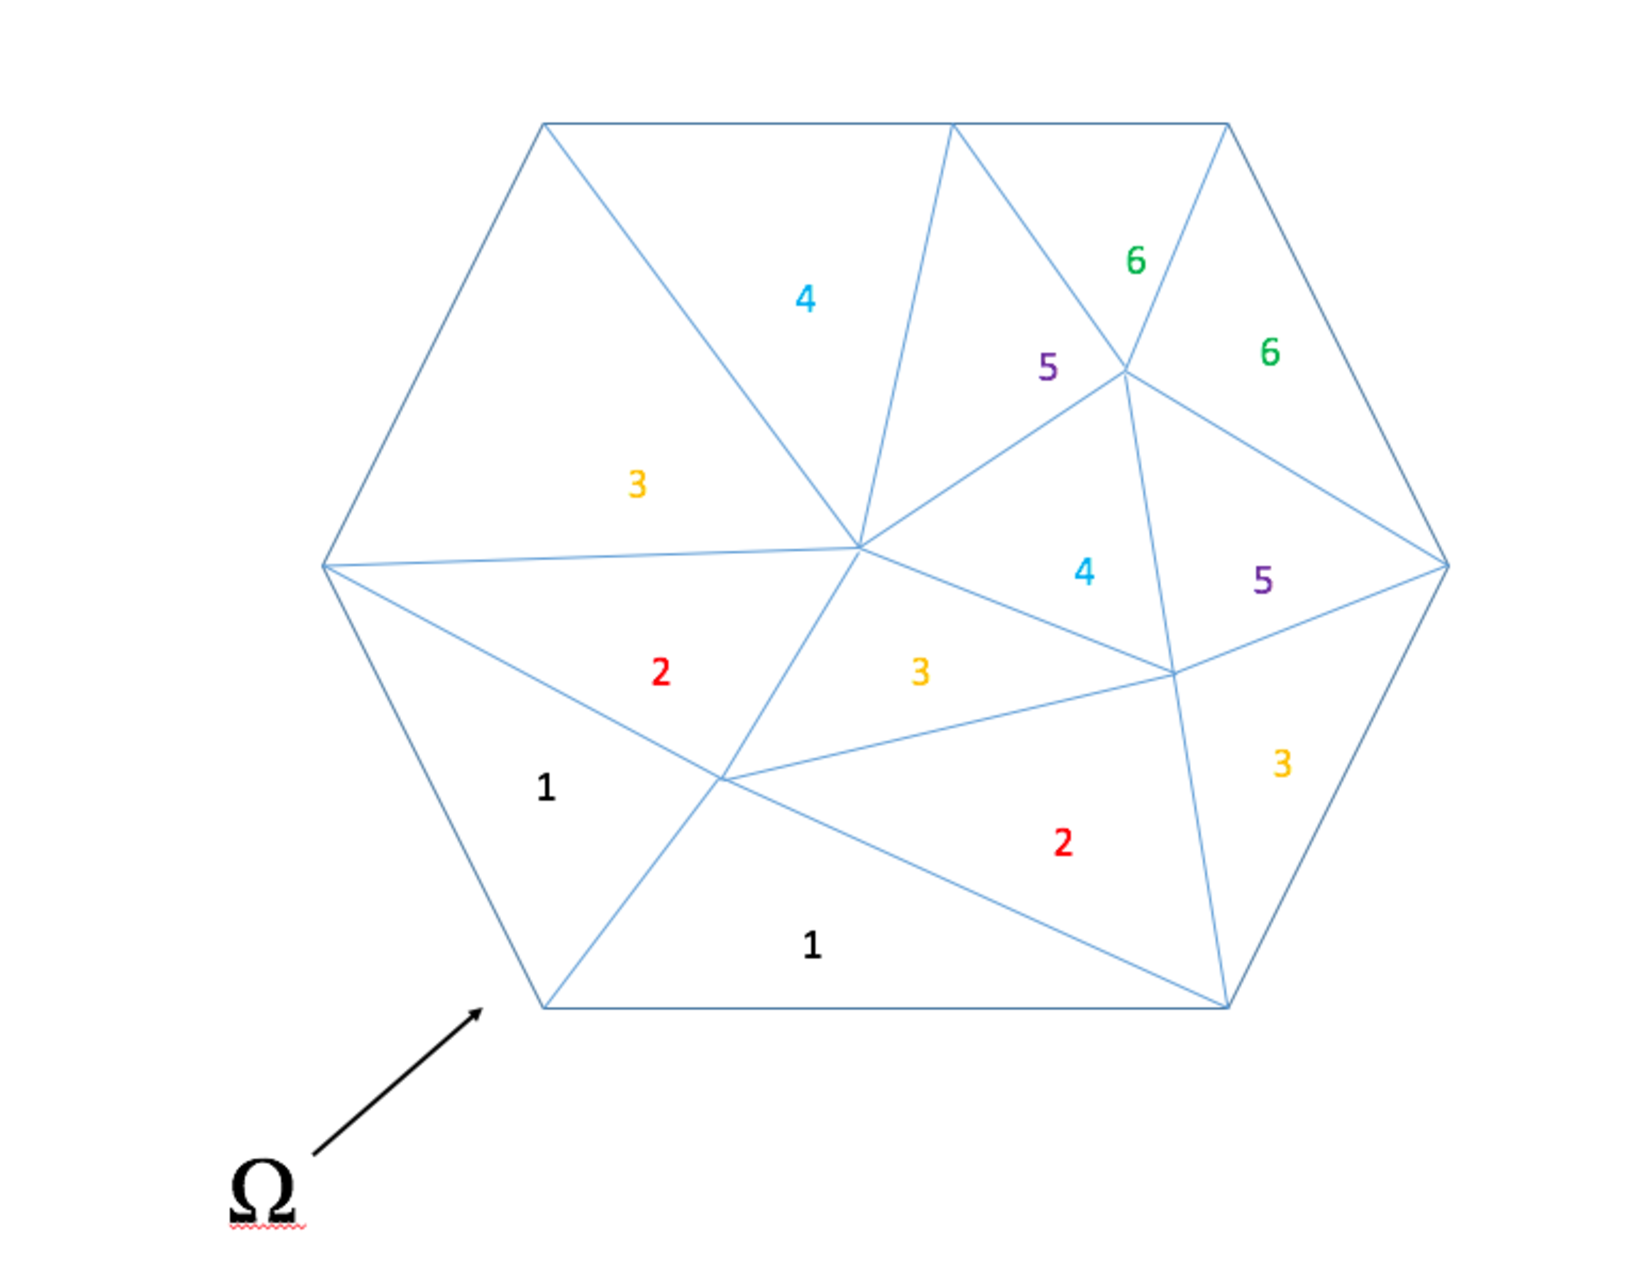
\includegraphics[scale = 0.27]{UnstructureMesh.pdf}
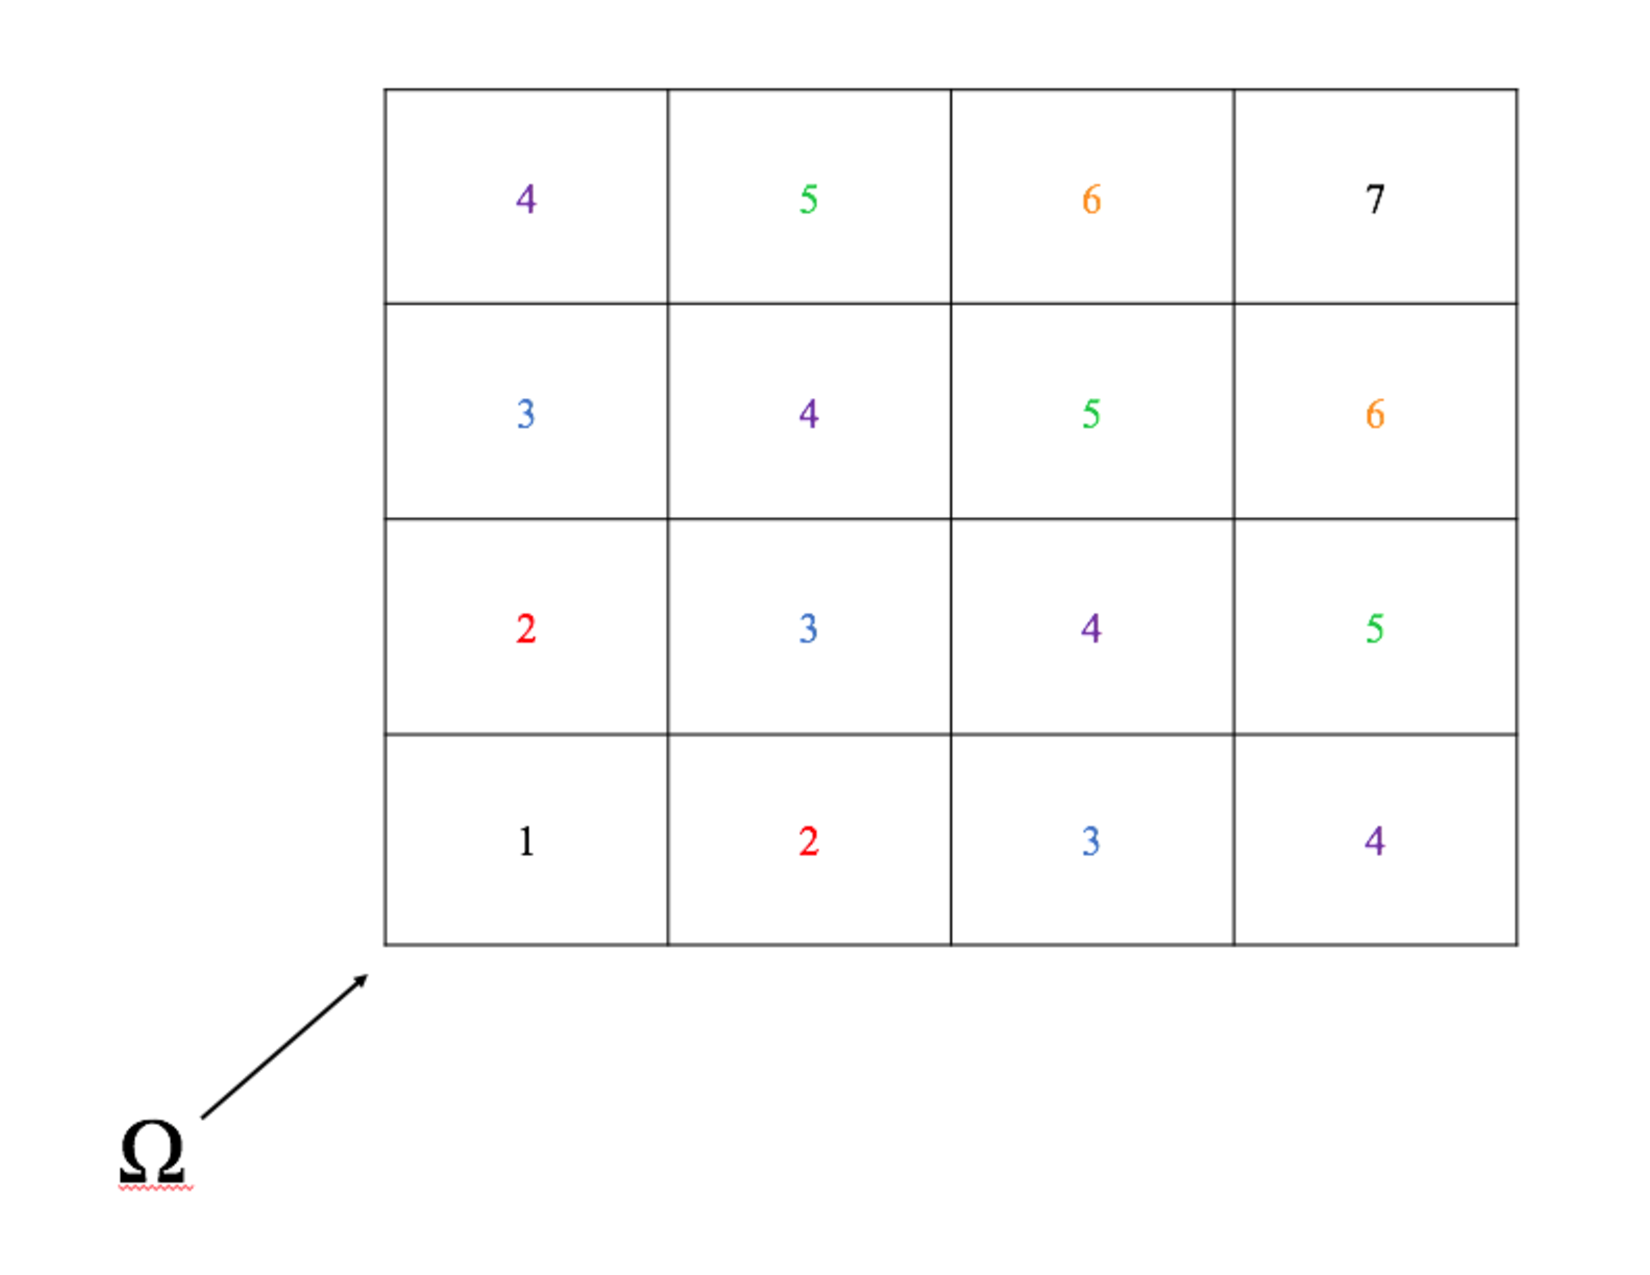
\includegraphics[scale = 0.27]{StructuredMesh.pdf}
\captionof{figure}{A demonstration of a sweep on a structured and unstructured mesh. }
\label{sweeps}
\end{minipage}
\smallskip

The number in each cell represents the order in which the cells are solved. All cells must receive the solution downwind from them before solving for their own solution. This dependency can be represented and stored as a task dependence graph, shown in Fig. \ref{tdg}.

\noindent\begin{minipage}{\textwidth}
\centering
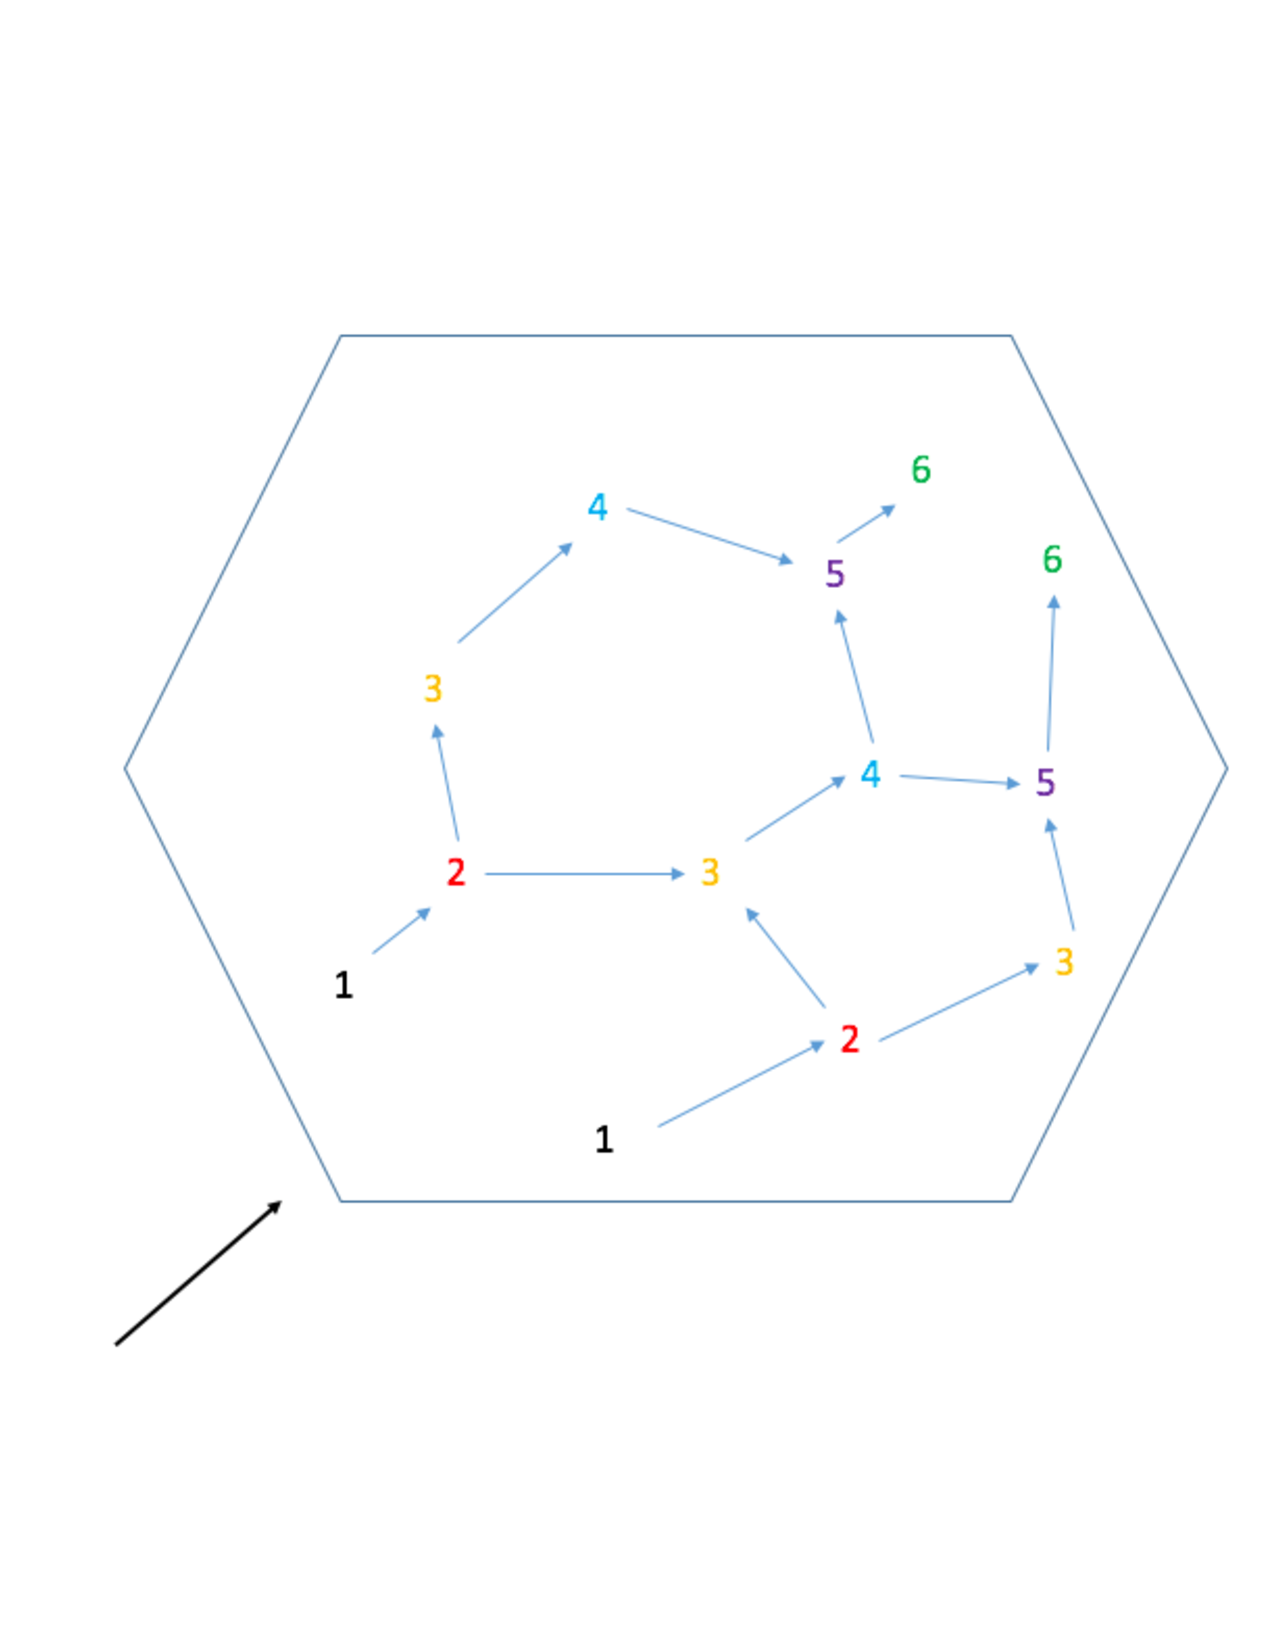
\includegraphics[scale = 0.5]{tdg.pdf}
\captionof{figure}{A task dependence graph of the unstructured mesh example in Fig. \ref{sweeps}.}
\label{tdg}
\end{minipage}
\smallskip

The concepts presented in this introduction are used to by PDT, Texas A\&M University's massively parallel deterministic transport code. It is capable of multi-group simulations and employs discrete ordinates for angular discretization. PDT features steady-state, time-dependent, criticality, and depletion simulations. It solves the transport equation for neutron, thermal, gamma, coupled neutron-gamma, electron, and coupled electron-photon radiation. PDT  has been shown to scale on logically Cartesian grids out to 750,000 cores. Logically Cartesian grids contain regular convex grid units that allow for vertex motion inside them, in order to conform to curved shapes. All work proposed in this document has been and will be implemented in PDT. 

%%%%%%%%%%%%%%%%%%%%%%%%%%%%%%%%%%%%%%%%%%
%%%%%%%%%%%%%%%%%%%%%%%%%%%%%%%%%%%%%%%%%%
\section{Parallelization of Transport Sweeps}
%%%%%%%%%%%%%%%%%%%%%%%%%%%%%%%%%%%%%%%%%%
%%%%%%%%%%%%%%%%%%%%%%%%%%%%%%%%%%%%%%%%%%

As mentioned in the previous section, a transport sweep is set up by overlaying a domain with a finite element mesh. The sweep then solves the transport equation cell by cell using a discontinuous finite element approach. The order of which cell to solve first is given by a task dependence graph, as shown in Fig. \ref{tdg}. The transport sweep can be solved in parallel in order to obtain the solution faster, as well as distribute the memory to many processors for memory intensive cases. In PDT, a transport sweep can be performed on a structured Cartesian mesh, and the work proposed utilizes transport sweeps on an unstructured mesh. Performing a transport sweep on an unstructured mesh presents two big challenges: performing a transport sweep on a massively parallel scale in an efficient manner and keeping non-concave sub-domains due to the nature of the transport sweep itself. PDT has already proven the ability to perform massively parallel transport sweeps on structured meshes. As part of previous efforts in PDT, researchers have come to outline three important properties for parallel sweeps. 

A parallel sweep algorithm is defined by three properties\cite{mpadams2013} :
\begin{itemize}
\item partitioning: dividing the domain among available processors
\item aggregation: grouping cells, directions, and energy groups into tasks
\item scheduling: choosing which task to execute if more than one is available
\end{itemize}

The basic concepts of parallel transport sweeps, partitioning, aggregation, and scheduling, are most easily described in the context of a structured transport sweep. A structured transport sweep takes place on a Cartesian mesh. Furthermore, the work proposed utilizes aspects of the structured transport sweep.

If $M$ is the number of angular directions per octant, $G$ is the total number of energy groups, and $N$ is the total number of cells, then the total fine grain work units is $8MGN$. The factor of 8 is present as $M$ directions are swept for all 8 octants of the domain. The finest grain work unit is the calculation of a single direction and energy groups unknowns in a single cell, or $\psi_{m,g}$ for a single cell.

In a regular grid, we have the  number of cells in each Cartesian direction: $N_x, N_y, N_z$. These cells are aggregated into ``cellsets''. If $M$ is the total number of angular directions, $G$ is the total number of energy groups, and $N$ is the total number of cells, then the total fine grain work units is $8MGN$. The factor of 8 is present as $M$ directions are swept for all 8 octants of the domain. The finest grain work unit is the calculation of a single direction and energy groups unknowns in a single cell, or $\psi_{m,g}$ for a single cell.

Fine grain work units are aggregated into coarser-grained units called \textit{tasks}. A few terms are defined that describe how each variable is aggregated.
\begin{itemize}
\item $A_x = \frac{N_x}{P_x}$, where $N_x$ is the number of cells in $x$ and $P_x$ is the number of processors in $x$
\item $A_y = \frac{N_y}{P_y}$, where $N_y$ is the number of cells in $y$ and $P_y$ is the number of processors in $y$
\item $N_g = \frac{G}{A_g}$
\item $N_m = \frac{M}{A_m}$
\item $N_k = \frac{N_z}{P_z A_z}$
\item $N_k A_x A_y A_z = \frac{N_x N_y N_z}{P_x P_y P_z}$
\end{itemize}

It follows that each process owns $N_k$ cell-sets (each of which is $A_z$ planes of $A_x A_y$ cells), $8N_m$ direction-sets, and $N_g$ group-sets for a total of $8N_m N_g N_k$ tasks.

One task contains $A_x A_y A_z$ cells, $A_m$ directions, and $A_g$ groups. Equivalently, a task is the computation of one cellset, one groupset, and one angleset. One task takes a stage to complete.  This is particularly important when comparing sweeps to the performance models. 

Equation ~\eqref{paralleleff} approximately defines parallel sweep efficiency. This can be calculated for specific machinery and partitioning parameters by substituting in values calculated using Eqs.~\eqref{nfill},~\eqref{nidle}, and ~\eqref{ntasks}.
\begin{equation}\label{paralleleff}
\begin{split}
\epsilon &= \frac{T_{\text{task}} N_{\text{tasks}}}{[N_{\text{stages}}] [T_{\text{task}} + T_{\text{comm}}]} \\
            &=\frac{1}{[1+\frac{N_{\text{idle}}}{N_{\text{tasks}}}][1 + \frac{T_{\text{comm}}}{T_{\text{task}}}]}
\end{split}
\end{equation}

Equations ~\eqref{Tcomm} and \ref{Ttask} show how $T_{\text{comm}}$ and $T_{\text{task}}$ are calculated:
\begin{equation}
T_{\text{comm}} = M_L T_{\text{latency}} + T_{\text{byte}} N_{\text{bytes}}
\label{Tcomm}
\end{equation}
\begin{equation}
T_{\text{task}} = A_x A_y A_z A_m A_g T_{\text{grind}}
\label{Ttask}
\end{equation}
where $T_{\text{latency}}$ is the message latency time, $T_{\text{byte}}$ is the time required to send one byte of message, $N_{\text{bytes}}$ is the total number of bytes of information that a processor must communicate to its downstream neighbors at each stage, and $T_{\text{grind}}$ is the time it takes to compute a single cell, direction, and energy group. $M_L$ is a latency parameter that is used to explore performance as a function of increased or decreased latency. If a high value of $M_L$ is necessary for the model to match computational results, improvements should be made in code implementation.

\subsection{KBA Partitioning for Structured Grids}

Several parallel transport sweep codes use KBA partitioning in their sweeping, such as Denovo \cite{denovo} and PARTISN \cite{partisn}. The KBA partitioning scheme and algorithm was developed by Koch, Baker, and Alcouffe \cite{partisn}.

The KBA algorithm traditionally chooses $P_z = 1, A_m = 1, G = A_g = 1, A_x = N_x/P_x, A_y = N_y/P_y$, with $A_z$ being the selectable number of z-planes to be aggregated into each task. With $N_k = N_z/A_z$, each processor performs $N_{\text{tasks}} = 8MN_k$ tasks. With the KBA algorithm, $2MN_k$ tasks are pipelined from a given corner of the 2D processor layout. The far corner processor remains idle for the first $P_x + P_y - 2 $ stages, which means that an octant-pair (or quadrant) sweep completes in $2MN_k + P_x + P_y - 2$ stages. If an octant-pair sweep does not begin until the previous pair's finishes, the full sweep requires $8MN_k + 4(P_x+P_y-2)$ stages, which means the KBA parallel efficiency is:
\begin{equation}
\varepsilon_{KBA} = \frac{1}{[1+\frac{4(P_x+P_y-2)}{8MN_k}][1+\frac{T_{\text{comm}}}{T_{\text{task}}}]}
\label{eKBA}
\end{equation}

%%%%%%%%%%%%%%%%%%%%%%%%%%%%%%%%%%%%%%%%%%%%%%%%%%%%%%%%%%%%%%%%%%%%%
\subsection{The Structured Transport Sweep in PDT}
%%%%%%%%%%%%%%%%%%%%%%%%%%%%%%%%%%%%%%%%%%%%%%%%%%%%%%%%%%%%%%%%%%%%%
The minimum possible number of stages for given partitioning parameters $P_i$ and $A_j$ is $2 N_{\text{fill}}+N_{\text{tasks}}$. $N_{\text{fill}}$ is both the minimum number of stages before a sweepfront can reach the center-most processors and the number needed to finish a direction's sweep after the center-most processors have finished. Equations~\eqref{nfill}, ~\eqref{nidle}, and~\eqref{ntasks} define $N_{\text{fill}}$, $N_{\text{idle}}$, and $N_{\text{tasks}}$:
\begin{equation}
N_{\text{fill}} = \frac{P_x + \delta_x}{2} - 1 + \frac{P_y + \delta_y}{2} - 1 + N_k (\frac{P_z + \delta_z}{2} - 1)
\label{nfill}
\end{equation}
\begin{equation}
N_{\text{idle}} = 2 N_{\text{fill}}
\label{nidle}
\end{equation}
\begin{equation}
N_{\text{tasks}} = 8 N_m N_g N_k
\label{ntasks}
\end{equation}
where $\delta_u$ is 1 for $P_u$ odd, and 0 for $P_u$ even.

Figure \ref{partitioning} shows three different partitioning schemes used in transport sweeps, KBA (which is defined in the previous section), volumetric non-overloaded, and volumetric overloaded. Volumetric non-overloaded requires that all cells owned by a processor are contiguous, where as volumetric non-overloaded partitioning does not have this restriction.  

\noindent\begin{minipage}{\textwidth}
\centering
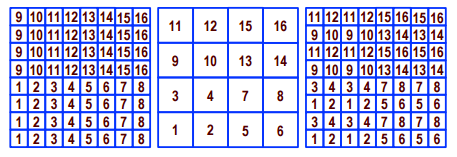
\includegraphics[scale = 1]{Partitioning.png}
\captionof{figure}{Three different partitioning schemes in 2D, from left to right: KBA, volumetric non-overloaded, and volumetric overloaded.}
\label{partitioning}
\end{minipage}

The overloaded volumetric partitioning proceeds as follows:

\begin{enumerate}
\item In a 2D (3D) domain, cellsets are divided into 4 (8) spatial quadrants (octants), with an equal number of cellsets in each  SQO (SQO is defined as a spatial quadrant or octant).
\item Assign 1/4 of the processors (1/8) in 3D to each SQO. 
\item Choose the individual overload factors $\omega_x, \omega_y, \text{and } \omega_z$ and individual processor counts $P_x, P_y, \text{and }P_z$, such that $\omega_x \omega_y \omega_z = \omega_r$ and $P_x P_y P_z = P$, with all $P_u$ even. $\omega_u$ is defined as the number of cellsets assigned to each $P_u$.
\item An array of $\omega_x\cdot\omega_y\cdot\omega_z$ ``tiles'' in each SQO. Each tile is an array of $1/2 P_x \cdot 1/2 P_y \cdot 1/2 P_z$ cellsets. These cellsets are mapped one-to-one to the $1/2 P_x \cdot 1/2 P_y \cdot 1/2 P_z$ processors assigned to the SQO, using the same mapping in each tile.
\end{enumerate}
Each tile has a logically identical layout of cellsets, and each processor owns exactly one cellset in each tile in its SQO. This makes each processor responsible for $\omega_r$ cellsets.

In order to properly outline the optimal scheduling rules, the variables $X,Y, \text{and } Z$ are defined as $P_u/2$ for each respective direction $u = x,y,z$. This splits up the processor layout into octants, where each processor has an index $(i,j,k)$ determining where it is in the layout. Tiles are also indexed and referred to in the same way with the notation $T(i,j,k)$. 

The optimal scheduling algorithm rules are as follows:
\begin{enumerate}
\item If $i \leq X$, then tasks with $\Omega_x > 0$ have priority, while for $i > X$, tasks with $\Omega_x < 0$ have priority.
\item If multiple ready tasks have the same sign on $\Omega_x$, apply rule 1 to $j,Y,\Omega_y$.
\item If multiple ready tasks have the same sign on $\Omega_x$ and $\Omega_y$, apply rule 1 to $k,Z, \Omega_z$. 
\item If multiple tasks are ready in the same octant, then priority goes to the cellset for which the priority octant has greatest downstream depth.
\item If multiple ready tasks are in the same octant and have the same downstream depth of graph in $x$, then priority goes to the cellset for which the priority octant has greatest downstream depth of graph in $y$.
\item If multiple ready tasks are in the same octant and have the same downstream depth of graph in $x$ and $y$, then priority goes to the cellset for which priority octant has greatest depth of graph in $z$.
\end{enumerate}
This ensures that each SQO orders the octants: the one it can start right away ($A$), three that have one sign difference from $A (B,C,$ and $D)$, three that have two sign differences ($\bar D, \bar C, \bar B$), and one in opposition to its primary ($\bar A$). For example, if octant $A$ is octant $(+x, +y, +z)$, then it's secondary octants (only one sign change at a time) would be octants $(-x, +y, +z)$, $(+x,-y,+z)$ and $(+x,+y,-z)$.

There are three constraints in order to achieve the optimal stage count. In these constraints, $M = \omega_g \omega_m/8$, which is the number of tasks per octant per cellset.
\begin{enumerate}
\item $ M \geq 2(Z-1)$
\item $\omega_z M \geq 2(Y-1)$
\item If $\omega_x > 1$, then $\omega_y \omega_z M \geq X$
\end{enumerate}
Constraint 1 ensures that there is no idle time between a processor finishing an octant's work in one tile and beginning that octant's work on the next tile in the same tile-column; processor $P(1,Y,1)$ finishing its tile $T(1,\omega_y,1)$ octant $C$ work and beginning its octant $B$ work; processor $P(X,1,1)$ finishing its tile $T(\omega_x,1,1)$ octant $D$ work and beginning its octant $B$ work. Constraint 2 ensures that there is no idle time time between a processor finishing an octant's work for one $z$ column of tiles and beginning that octant's work on the next column; processor $P(X,1,1)$ finishing its tile $T(\omega_x,1,1)$ octant D work available to it and beginning its octant $C$ work. Constraint 3 ensures that there is no idle time between a processor finishing an octant's work for one $yz$ plane of tiles and beginning that octant's work in the next plane.

As a result of these constraints, there is no idle time for a variety of situtations. At large processor counts, the product $\omega_m \omega_g$ must be large, which requires $N_m N_g$ be large. This means that a weak scaling series refined only in space, but only coarsely refined in angle and energy, will eventually fail the constraints.

The optimal efficiency formula changes slightly from the KBA and hybrid KBA partitioning method in order to account for the overload factors. The only change is in the $\frac{N_{idle}}{N_{tasks}}$ term, as shown in Eq. ~\eqref{overloadpartitioning}. 
\begin{equation}
\varepsilon_{opt} = \frac{1}{[1+\frac{P_x+P_y+P_z-6}{\omega_g \omega_m \omega_r}][1+\frac{T_{\text{comm}}}{T_{\text{task}}}]}
\label{overloadpartitioning}
\end{equation}


%%%%%%%%%%%%%%%%%%%%%%%%%%%%%%%%%%%%%%%%%%
\subsection{The Unstructured Transport Sweep}
%%%%%%%%%%%%%%%%%%%%%%%%%%%%%%%%%%%%%%%%%%
In an unstructured mesh, the number of cells cannot be described in the same way as an unstructured mesh. In PDT specifically we initially subdivide the domain into subsets, which are just rectangular subdomains. Within each subset, an unstructured mesh is created. This creates a pseudo-regular grid. These subsets become the $N_x, N_y, N_z$ equivalent for an unstructured mesh. The spatial aggregation in a PDT unstructured mesh is done by aggregating subsets into cellsets. 

While the structured PDT transport sweep has scaled well out to 750,000 cores, similar levels of parallel scaling have not been achieved using unstructured sweeps yet. Pautz proposed a new list scheduling algorithm has been constructed for modest levels of parallelism (up to 126 processors)\cite{Pautz} .

There are three requirements for a sweep scheduling algorithm to have. First, the algorithm should have low complexity, since millions of individual tasks are swept over in a typical problem. Second, the algorithm should schedule on a set of processors that is small in comparison to the number of tasks in the sweep graph. Last, the algorithm should distribute work in the spatial dimension only, so that there is no need to communicate during the calculation of the scattering source. 

Here is the pseudocode for the algorithm:

\begin{verbatim}
Assign priorities to every cell-angle pair
Place all initially ready tasks in priority queue
While (uncompleted tasks)
    For i=1,maxCellsPerStep
       Perform task at top of priority queue
       Place new on-processor tasks in queue
    Send new partition boundary data
    Receive new partition boundary data
    Place new tasks in queue 
\end{verbatim}

An important part of the algorithm above is the assigning priorities to tasks. Specialized prioritization heuristics generate partition boundary data as rapidly as possible in order to minimize the processor idle time. 

Nearly linear speedups were obtained on up to 126 processors. Further work is being done for scaling to thousands of processors. 

\subsubsection{Cycle Detection}

A cycle is a loop in a directed graph and they can occur commonly in unstructured meshes. However, they do not exist in 2D triangular extruded problems and, because our domain partitioning is convex, arbitrary degenerate polygons appearing on subdomain boundaries will not produce cycles. Even though they are not applicable to this application of unstructured transport sweeps, they are discussed here for completeness.

Cycles can cause hang time in the problem, as a processor will wait for a message that might will never come. This means that the computation for one or more elements will never be completed. The solution to this is to ``break'' any cycles that exist by removing an edge of the task dependence graph (TDG). Old flux information is used on a particular element face in the domain. Most of the time, the edge removed is oriented obliquely with respect to the radiation direction. 

Algorithms for finding cycles are called \textit{cycle detection} algorithms. This must be done efficiently in parallel, both because the task dependence graph is distributed and because the finite element grid may be deforming every timestep and changing the associated TDG.

Cycle detection utilizes two operations: trim and mark. Trimming identifies and discards elements which are not in cycles. At the beginning of cycle detection, graphs are trimmed in the downwind direction, then the remaining graphs are trimmed in the upwind direction. A pivot vertex is then selected in each graph. Graph vertices are then marked as upwind, downwind, or unmarked. Then, if any vertices are both upwind and downwind, the cycle is these vertices plus the pivot vertex. An edge is removed between 2 cycle vertices, and 4 new graphs are created: a new cycle, the upwind vertices without the cycle, the downwind vertices without the cycle, and a set of unmarked vertices. This recursively continues until all cycles are eliminated.

\section{Motivation and Proposed Method for Load Balancing Unstructured Meshes in PDT}

The capability for PDT to generate and run on an unstructured mesh is important because it allows us to run problems without having to conform our mesh to the problem as much. The idea is to have a logically Cartesian grid (creating orthogonal ``subsets") with an unstructured mesh inside each subset. These logically Cartesian subdomains are obtained using cut planes in 3D and cut lines in 2D. Figure \ref{grid} demonstrates this functionality, with the first two subsets meshed using the Triangle Mesh Generator\cite{triangle}, a 2D mesh generator. 

\noindent\begin{minipage}{\textwidth}
\centering
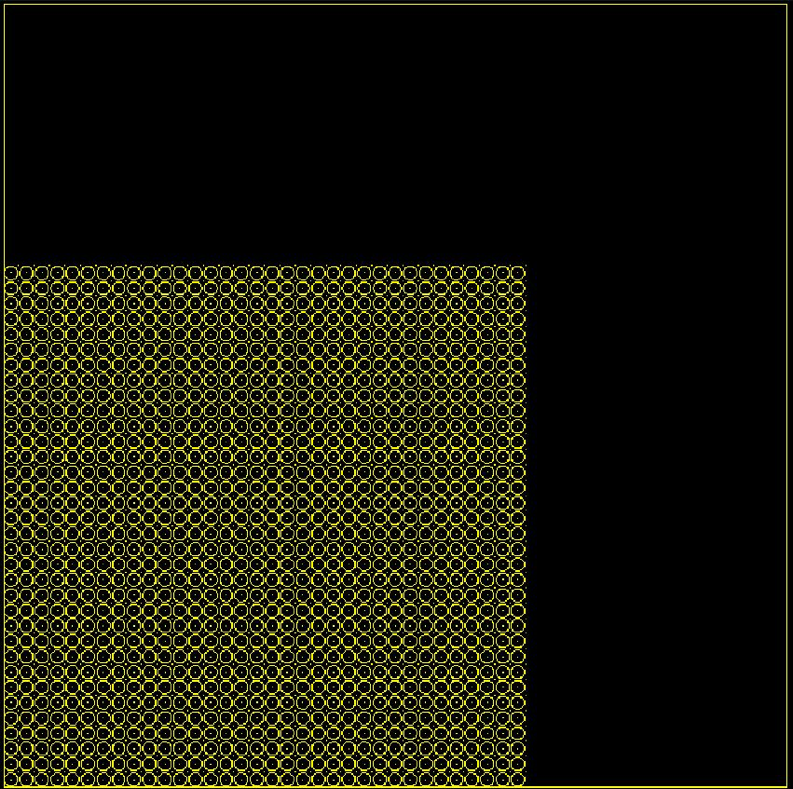
\includegraphics[scale = 0.5]{lattice.png}
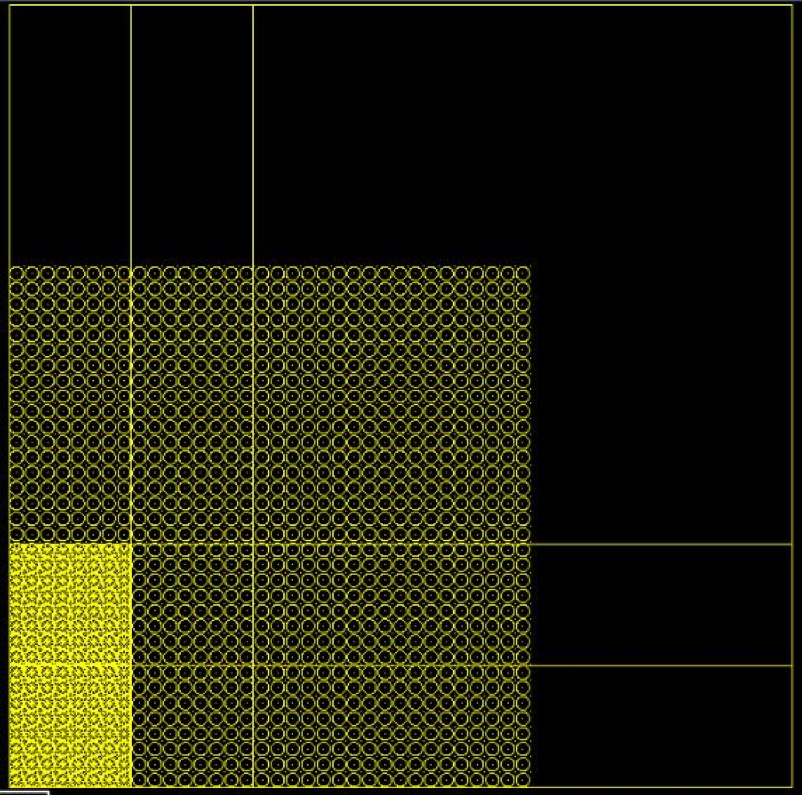
\includegraphics[scale = 0.5]{subsetlattice.png}
\captionof{figure}{A PSLG describing a fuel lattice, and with a orthogonal ``subset" grid imposed on on the PSLG.}
\label{grid}
\end{minipage}

This orthogonal grid is superimposed and each subset is meshed in parallel.  Subsets are now the base structured unit when calculating our parallel efficiency. Discontinuities along the boundary are fixed by ``stitching'' hanging nodes, creating degenerate polygons along subset boundaries. Because PDT's spatial discretization employs Piece-Wise Linear Discontinuous (PWLD) finite element basis functions, there is no problem solving on degenerate polygons. 

When using the unstructured meshing capability in PDT, the input geometry is described by a Planar Straight Line Graph (PSLG). After superimposing the orthogonal grid, a PSLG is created for each subset, and meshed. Because the input's and each subset's PSLG must be described and meshed in 2D, the mesh can be extruded in the $z$ dimension in order to give us the capability to run on 3D problems. Obviously, this is not as good as a unstructured tetrahedral mesh, but for many problems, it is a great capability to have. 

When discussing the parallel scaling of transport sweeps, a load balanced problem is of great importance. A load balanced problem has an equal number of degrees of freedom per processor. Load balancing is important in order to minimize idle time for all processors by equally distributing (as much as possible) the work each processor has to do.  For the purposes of unstructured meshes in PDT, we are looking to ``balance'' the number of cells. Ideally, each processor will be responsible for an equal number of cells. 

If the number of cells in each subset can be reasonably balanced, then the problem is effectively load balanced. The Load Balance algorithm described below details how the subsets will be load balanced. In summary, the procedure of the algorithm involves moving the initially user specified $x$ and $y$ cut planes, re-meshing, and iterating until a reasonably load balanced problem is obtained. 

\noindent\begin{minipage}{\textwidth}
\textbf{Load Balance:} A load balancing algorithm that equalizes the number of triangles per subset. \\
\rule{\textwidth}{0.4pt}
\begin{algorithmic}
\STATE  $I,J$ subsets specified by user

\STATE Mesh all subsets

\STATE  $N_{tot} = $ total number of triangles
\STATE  $N_{ij} = $ number of triangles in subset $ij$

\STATE $f =\underset{ij}{\text{max}}(N_{ij})/\frac{N_{tot}}{I\cdot J}$

\COMMENT {//Check if all subsets meet the tolerance}
\IF {$f < \text{tol}_{\text{subset}}$}
	\STATE DONE with load balancing
\ELSE
	\STATE $f_I = \underset{i}{\text{max}}[\sum_{j} N_{ij}]/\frac{N_{tot}}{I}$
	
	\STATE $f_J = \underset{j}{\text{max}}[\sum_{i} N_{ij}]/\frac{N_{tot}}{J}$
	
	\IF {$f_I > \text{tol}_{\text{row}}$}
		\STATE \textbf{Redistribute}($X_i$)
	\ENDIF
	
	\IF{$f_J > \text{tol}_{\text{col}}$}
		\STATE \textbf{Redistribute}($Y_j$)
	\ENDIF 
	
	\IF {redistribution occured}
		\STATE REMESH and repeat algorithm
	\ENDIF
	
\ENDIF

\IF {There is still a discrepancy amongst subsets}
     \STATE Move cutplane segments on the subset level and remesh (may require changes to scheduling algorithm)
\ENDIF
\end{algorithmic}
\rule{\textwidth}{0.4pt}
\end{minipage}

\bigskip

\noindent\begin{minipage}{\textwidth}
\textbf{Redistribute:} A function that moves cut lines in either X or Y. \\
\rule{\textwidth}{0.4pt}
\begin{algorithmic}
\STATE \textbf{Input:}CutLines (X or Y vector that stores cut lines). 
\STATE \textbf{Input:} num\_tri\_row or num\_tri\_col, a pArray containing number of triangles in each row or column 
\STATE \textbf{Input:} The total number of triangles in the domain, $N_{tot}$

\STATE stapl::array\_view num\_tri\_view, over num\_tri\_row/column
\STATE stapl::array\_vew offset\_view

\STATE stapl::partial\_sum(num\_tri\_view) \COMMENT {Perform prefix sum}

\COMMENT {We now have a cumulative distribution stored in offset\_view}

\FOR {$i = 1$ :CutLines.size()-1}

	\STATE vector $<$double$>$ pt1 = [CutLines(i-1), offset\_view(i-1)]
	\STATE vector $<$double$>$ pt2 = [CutLines(i), offset\_view(i)]
	\STATE ideal\_value = $i\cdot \frac{N_{tot}}{\text{CutLines.size()}-1}$
	\STATE X-intersect(pt1,pt2,ideal\_value) \COMMENT{Calculates the X-intersect of the line formed by pt1 and pt2 and the line y = ideal\_value.}
	\STATE CutLines(i) = X-intersect
\ENDFOR
\end{algorithmic}
\rule{\textwidth}{0.4pt}
\end{minipage} 

\section{Results}

\tcr{give the dimension of your domains. I suppose since XS are in 1/cm, the domain and the trinalge areas are in cm2 but say it}

The following sections will showcase the new unstructured meshing capability both in 2D and 3D, the metric behavior and convergence for three test cases, and solution verification for pure absorber and pure scatterer 2D slab problems. 

\subsection{2D and 2D Extruded Meshing Capability}

\tcr{not sure what you want to start with what could be the best results. Why not build up momentum and show this as the grand finale?}


Figure \ref{IM12D} showcases the 2D meshing capability, and Fig. \ref{IM13D} showcases the same mesh extruded in the z  direction.



\subsection{Test Cases for Metric Behavior and Convergence}

In order to showcase the behavior of the load balancing metric \tcr{it would be good to provide the equation number for the metric, for clarity}, three test cases are presented. Figure \ref{opp} shows the first test case, a large domain with two pins in opposite corners of the domain. Figure \ref{same} shows the same size domain but with the pins on the same side.These are two theoretically very unbalanced cases, as geometrically there are two features located distantly from each other with an empty geometry throughout the rest of the domain. Figure \ref{lattice} shows a lattice and reflector, which due to it's denser and repeated geometry, theoretically is a more balanced problem. 

A series of 162 inputs was constructed for each case. Table \ref{study} shows the the parameters that will change in each input. The maximum triangle area varied from the coarsest possible to 0.01, and the number of subsets, $N$, varies from 2x2 to 10x10. 

\noindent\begin{minipage}{\textwidth}
\captionof{table}{The parameters of the 162 inputs for each case.}
\centering
\begin{tabular}{c c c c c c c c c c }
\textbf{Area test is coarse so fuck it} &  \textbf{N = 4}	& \textbf{N = 9}	& \textbf{N = 16}	& \textbf{N = 25}	&\textbf{N = 36}&	\textbf{N = 49}	& \textbf{N = 64	}& \textbf{N = 81}	& \textbf{N = 100}  \\
\textbf{Coarse} & 		&		& 	        & 		&          &                   &               &             &                \\
\textbf{1.8	} & 				& 			&         &         &      &          &         &         &          \\
\textbf{1.6	} & 				& 			&         &         &      &          &         &         &          \\
\textbf{1.4	} & 				& 			&         &         &      &          &         &         &          \\
\textbf{1.2	} & 				& 			&         &         &      &          &         &         &          \\
\textbf{1}    & 				& 		  &         &         &      &          &         &         &          \\
\textbf{0.8	} & 				& 			&         &         &      &          &         &         &          \\
\textbf{0.6	} & 				& 			&         &         &      &          &         &         &          \\
\textbf{0.4	} & 				& 			&         &         &      &          &         &         &          \\
\textbf{0.2	} & 				& 			&         &         &      &          &         &         &          \\
\textbf{0.1	} & 				& 			&         &         &      &          &         &         &          \\
\textbf{0.08} & 				& 			& 	      &         &      &          &         &         &          \\
\textbf{0.06} & 				& 			& 	      &         &      &          &         &         &          \\
\textbf{0.05} & 				& 			& 	      &         &      &          &         &         &          \\
\textbf{0.04} & 				& 			& 	      &         &      &          &         &         &          \\
\textbf{0.03} & 				& 			& 	      &         &      &          &         &         &          \\
\textbf{0.02} & 				& 			& 	      &         &      &          &         &         &          \\
\textbf{0.01} & 				& 			& 	      &         &      &          &         &         &          \\
\end{tabular}
\label{study}
\end{minipage}

\tcr{do not call first and second poly files. Be creative, come up with names for the examples, be it only Example 1,2,3, or Example I,II,III, or Example A, B, C ....}

  \noindent\begin{minipage}{\textwidth}
\centering
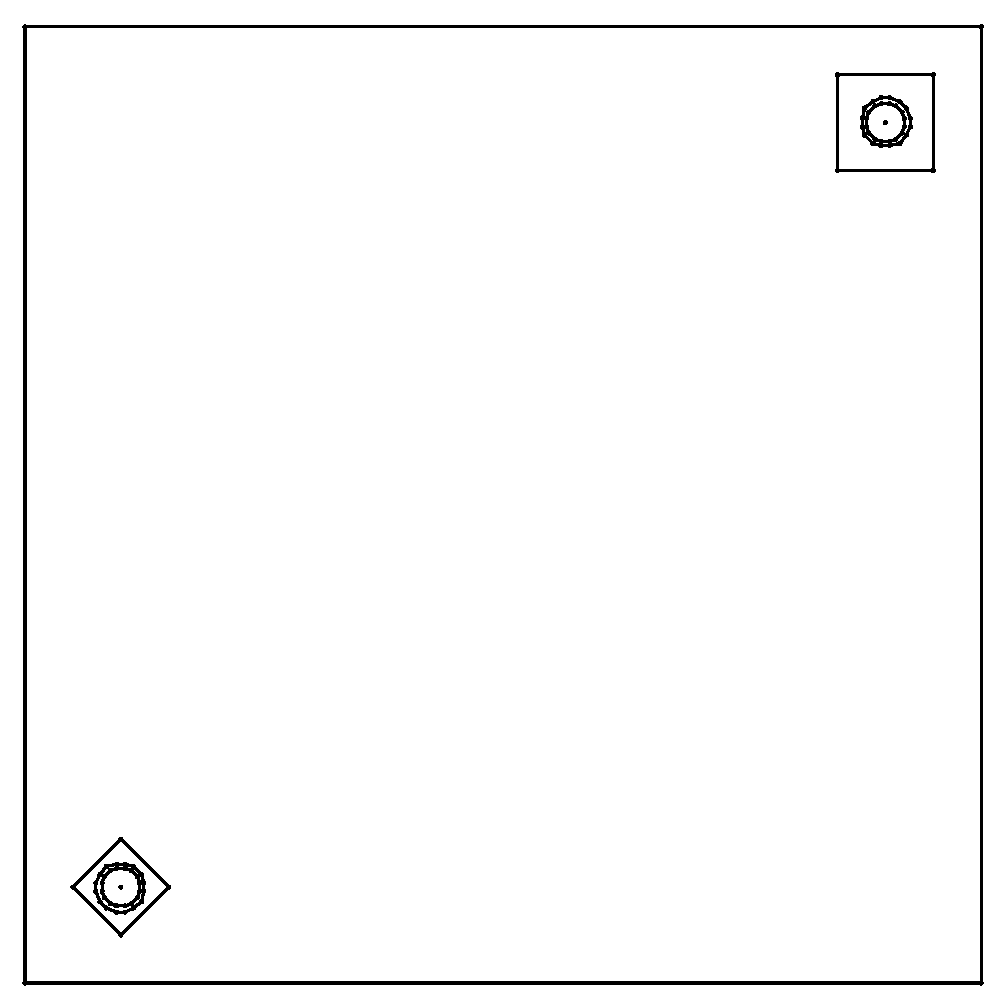
\includegraphics[scale = 0.5]{unbalanced_lattice.eps}
\captionof{figure}{The first .poly file used in order to test effectiveness and convergence of the load balancing metric.}
\label{opp}
\end{minipage}

\noindent\begin{minipage}{\textwidth}
\centering
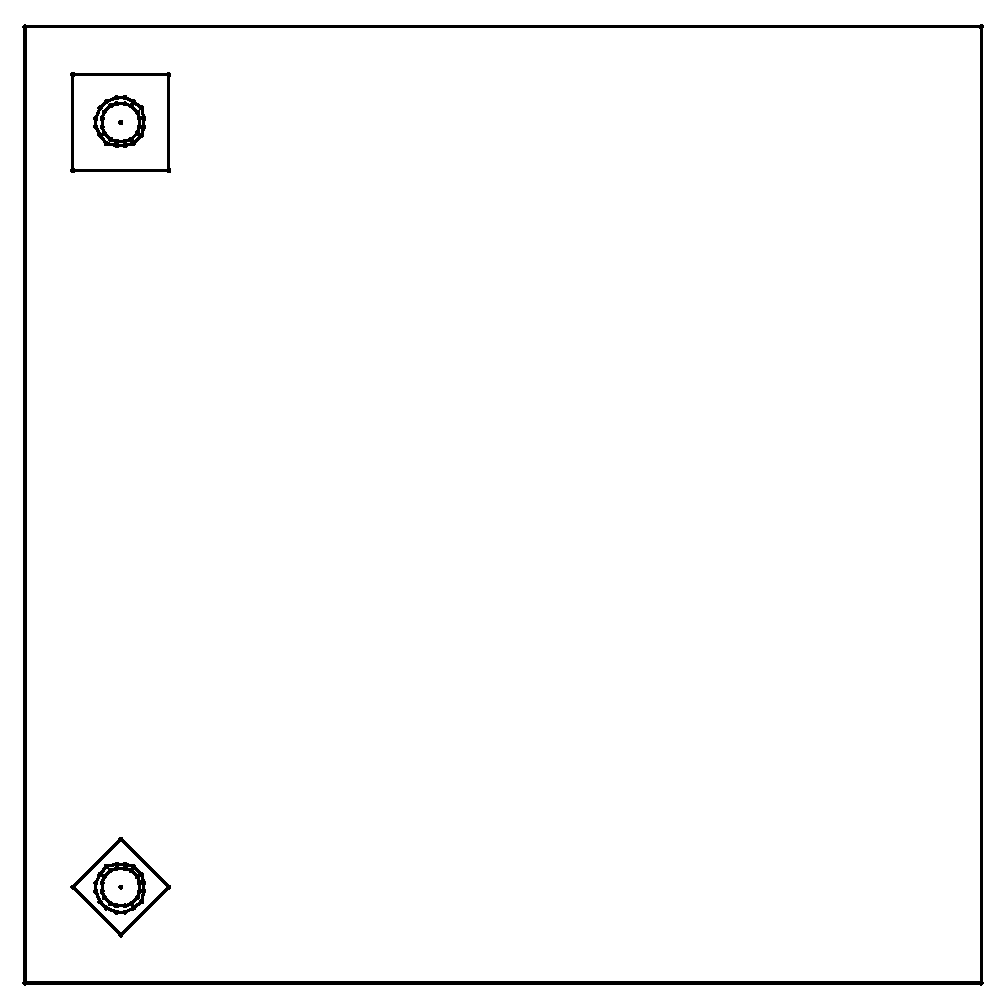
\includegraphics[scale = 0.5]{unbalanced_pins_same_side.eps}
\captionof{figure}{The second .poly file used in order to test effectiveness and convergence of the load balancing metric.}
\label{same}
\end{minipage}


\noindent\begin{minipage}{\textwidth}
\centering
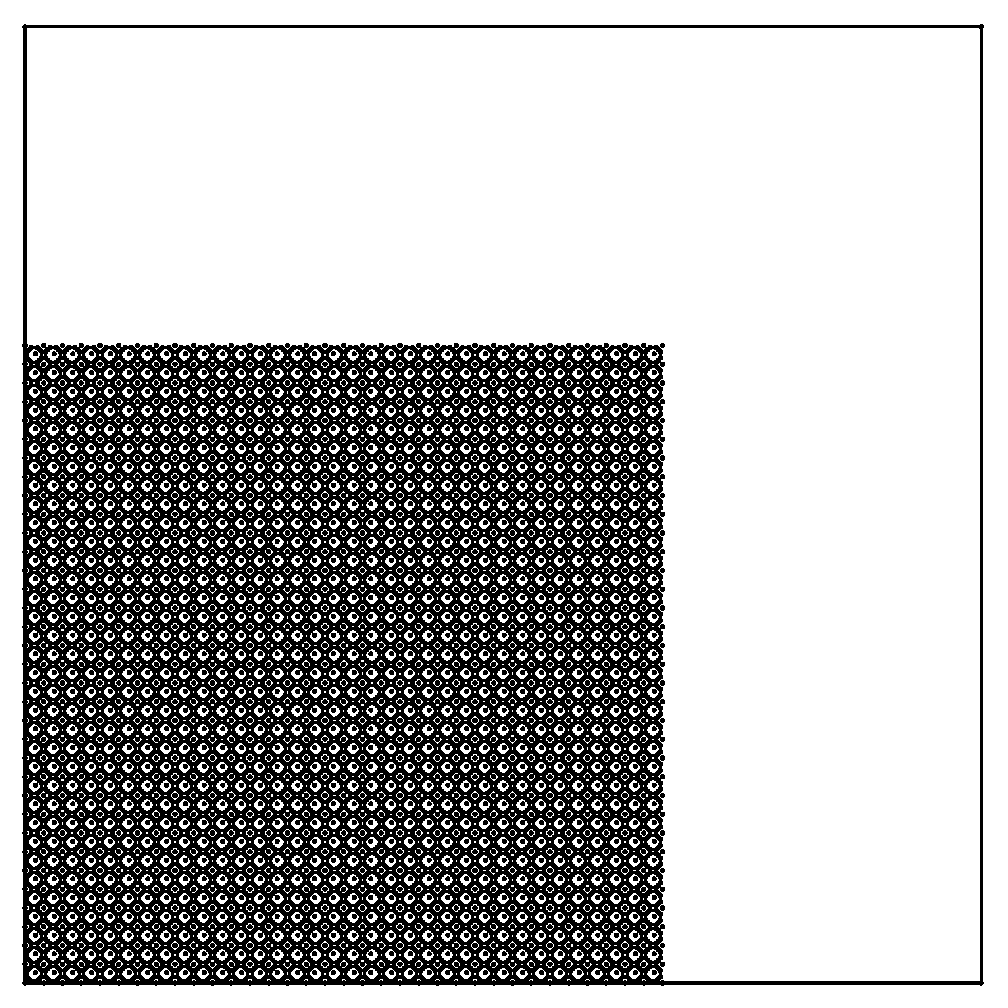
\includegraphics[scale = 0.5]{lattice-12-shifted.eps}
\captionof{figure}{The third .poly file used in order to test effectiveness and convergence of the load balancing metric.}
\label{lattice}
\end{minipage}

\subsection{Metric Behavior and Convergence}

For each test case, the 162 input parameters outlined in Table \ref{study} are run twice, once with no load balancing iterations, and once with ten load balancing iterations. The best metric is reported and recorded. Three figures for each test cases are presented below: the first figure will show the metric behavior for no iterations, the second figure will show the metric behavior for each input run with ten load balancing iterations, and the third figure will show a ratio of the ten iteration runs over the no iteration runs.

Figure \ref{oppnoiter} shows the metric behavior for Fig. \ref{opp}. The maximum metric value is 24.7650, and occurs when Fig. \ref{opp} is run with 8x8 subsets and a maximum triangle area of 1.6 cm\textsuperscript{2}. The minimum metric value is 1.0016 and occurs when Fig. \ref{opp} is run with 4x4 subsets and a maximum triangle area of 0.04 cm\textsuperscript{2}. 

\noindent\begin{minipage}{\textwidth}
\centering
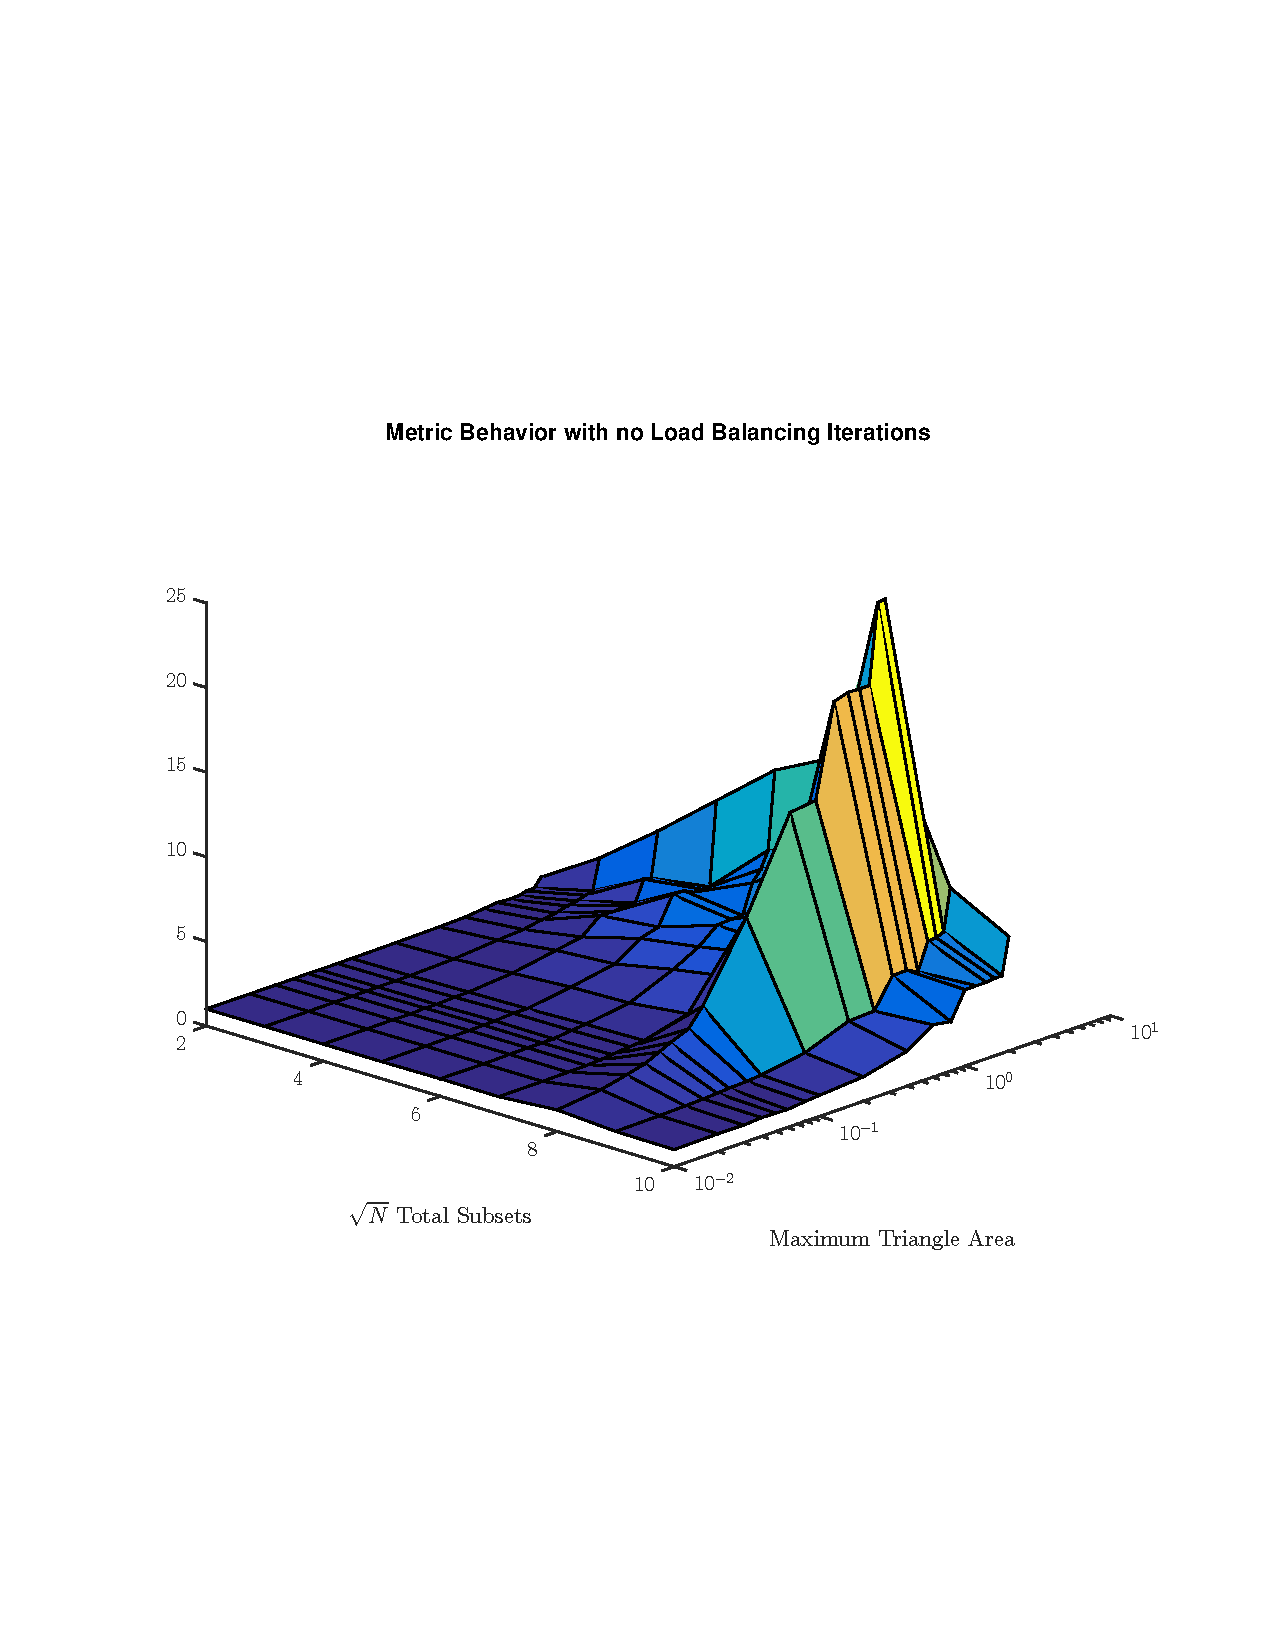
\includegraphics[scale=0.75, trim = 0cm 2cm 0cm 3cm,clip]{OppNoIter.pdf}
\captionof{figure}{The metric behavior of the first test case run with no load balancing iterations.}
\label{oppnoiter}
\end{minipage}

Figure \ref{oppiter} shows the metric behavior for Fig. \ref{opp}. The maximum metric value is 5.0538 and occurs when Fig. \ref{opp} is run with 10x10 subsets and a maximum triangle area of 1.2 cm\textsuperscript{2}. The minimum metric value is 1.0017 and occurs when Fig. \ref{opp} is run with 4x4 subsets and a maximum triangle area of 0.04 cm\textsuperscript{2}.

\noindent\begin{minipage}{\textwidth}
\centering
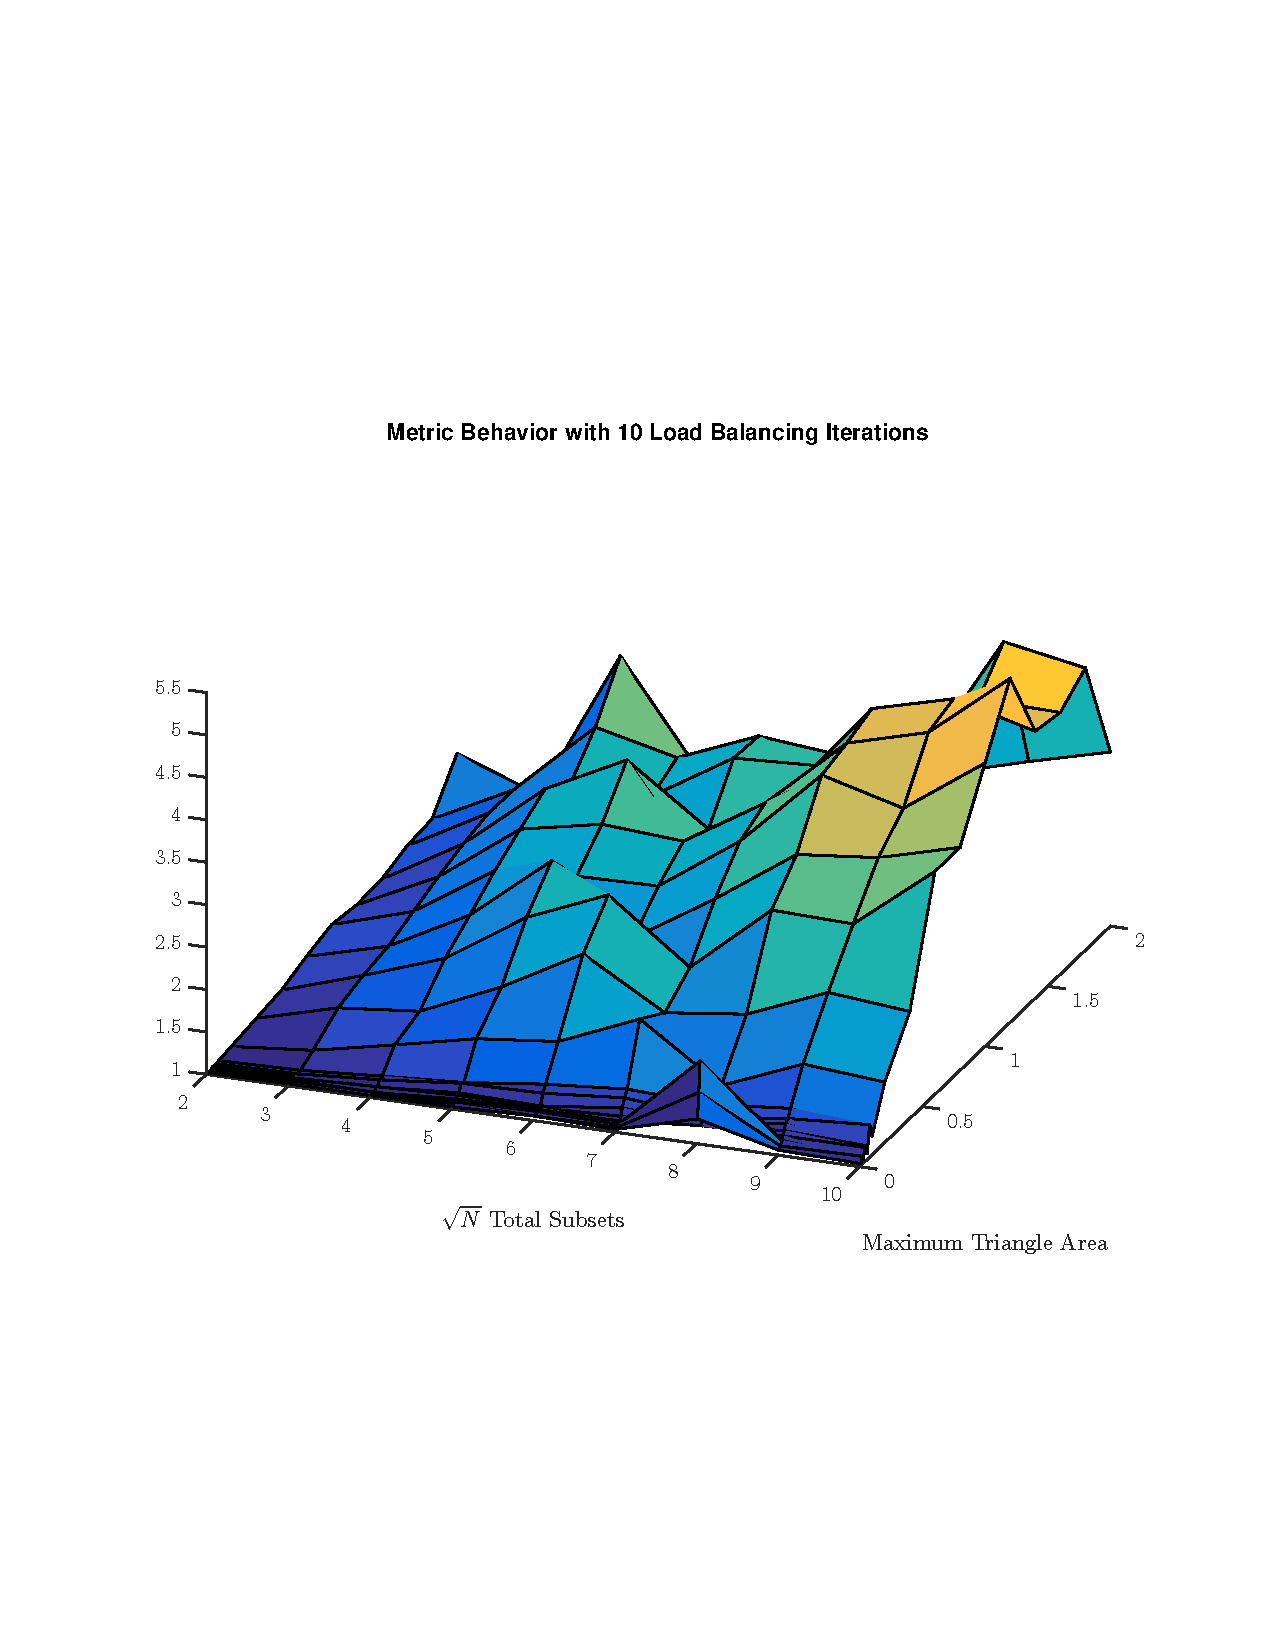
\includegraphics[scale=0.83, , trim = 0cm 2cm 0cm 3cm,clip]{OppIter.pdf}
\captionof{figure}{The metric behavior of the first test case run with 10 load balancing iterations.}
\label{oppiter}
\end{minipage}

Figure \ref{oppdiff} shows the difference in metric behavior for Fig. \ref{opp}. This difference is calculated by dividing the metric with no iterations by the metric with 10 iterations. The maximum improvement has a value of 0.1097 and occurs for Fig. \ref{opp} is run with 8x8 subsets with a maximum triangle area of 1.6 cm\textsuperscript{2}. The minimum improvement has a value of very close to 1.0 and occurs for many of the inputs. 

\noindent\begin{minipage}{\textwidth}
\centering
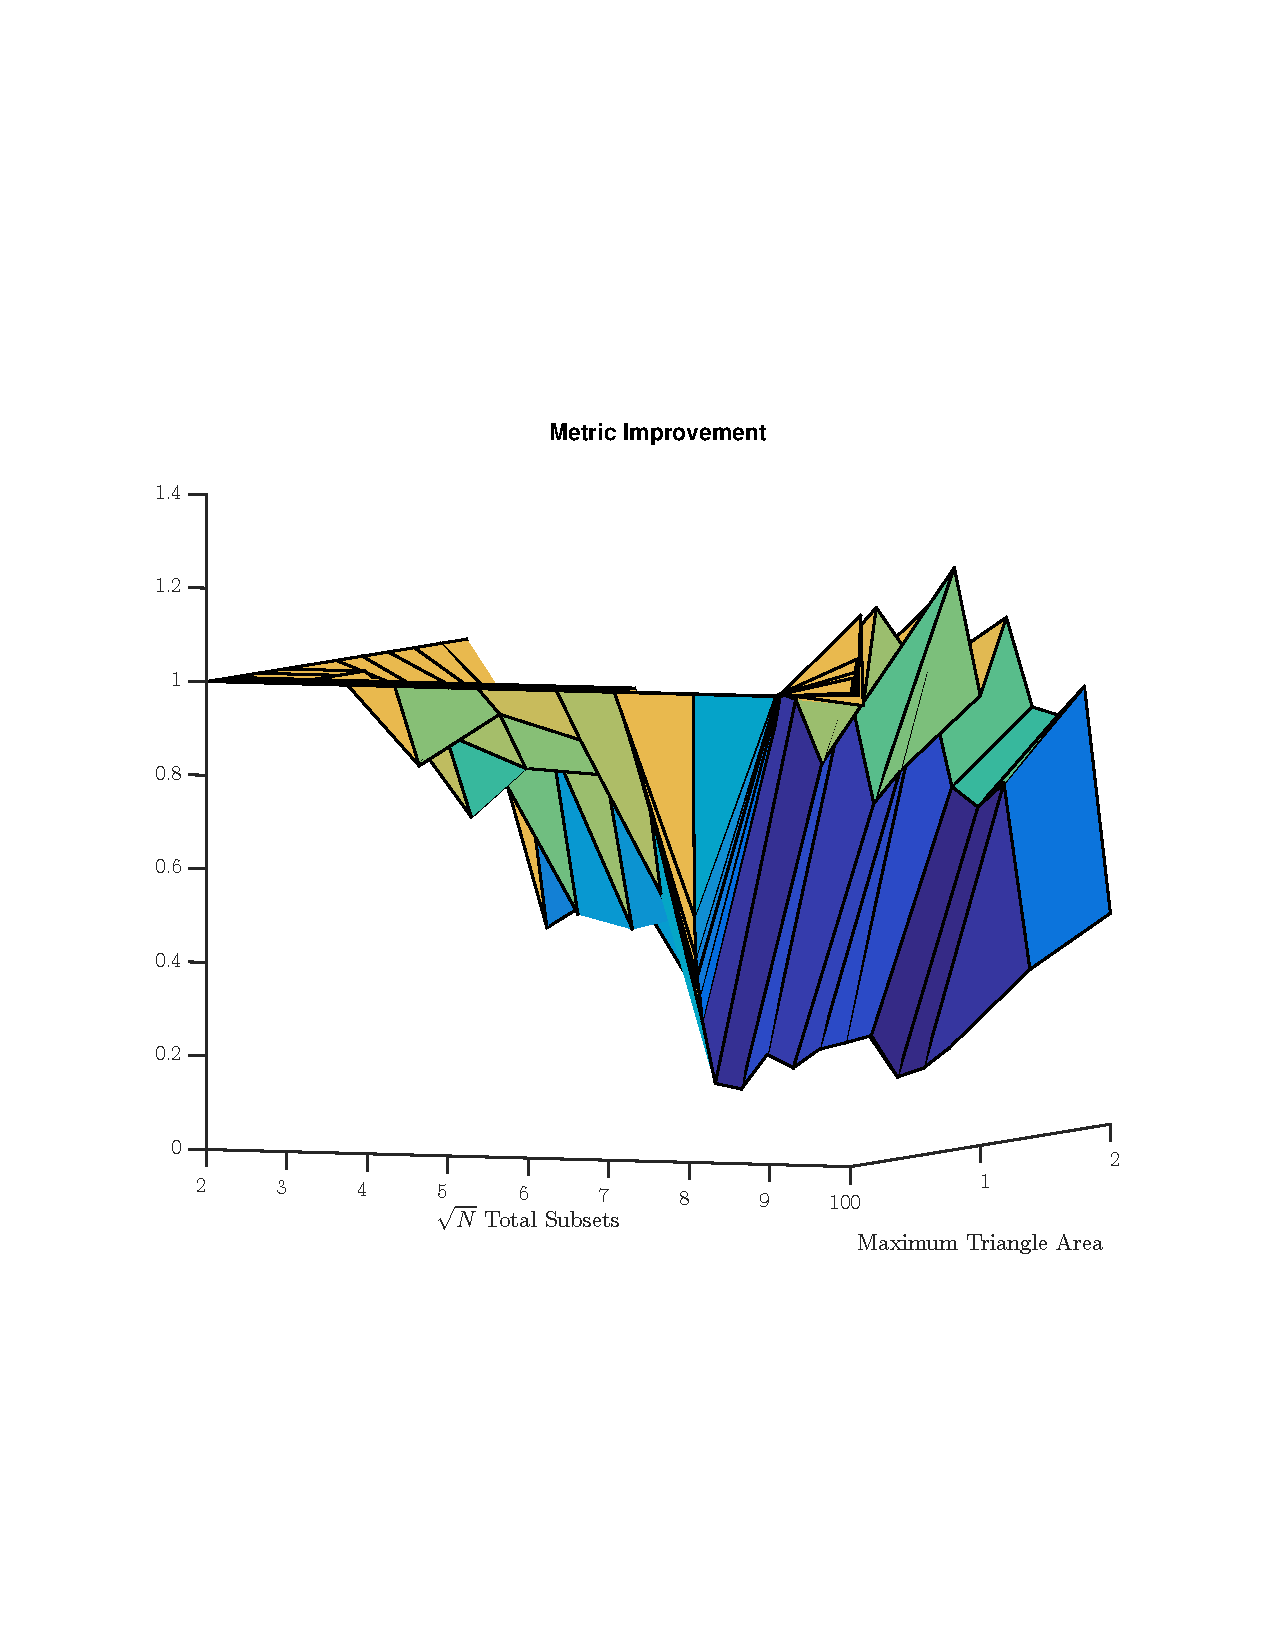
\includegraphics[scale=0.78, trim = 0cm 2cm 0cm 3cm,clip]{OppDiff.pdf}
\captionof{figure}{The difference in metric behavior between no iteration and 10 iterations. The closer the z-value to zero, the better the improvement.}
\label{oppdiff}
\end{minipage}

Figure \ref{samenoiter} shows the metric behavior for Fig. \ref{same}. The maximum metric is 22.6654 and occurs when Fig. \ref{same} is run with 8x8 subsets with a maximum triangle area of 1.8 cm\textsuperscript{2}. The minimum metric is 1.0024 and occurs when Fig. \ref{same} is run with 2x2 subsets with a maximum triangle are of 0.01 cm\textsuperscript{2}.

\noindent\begin{minipage}{\textwidth}
\centering
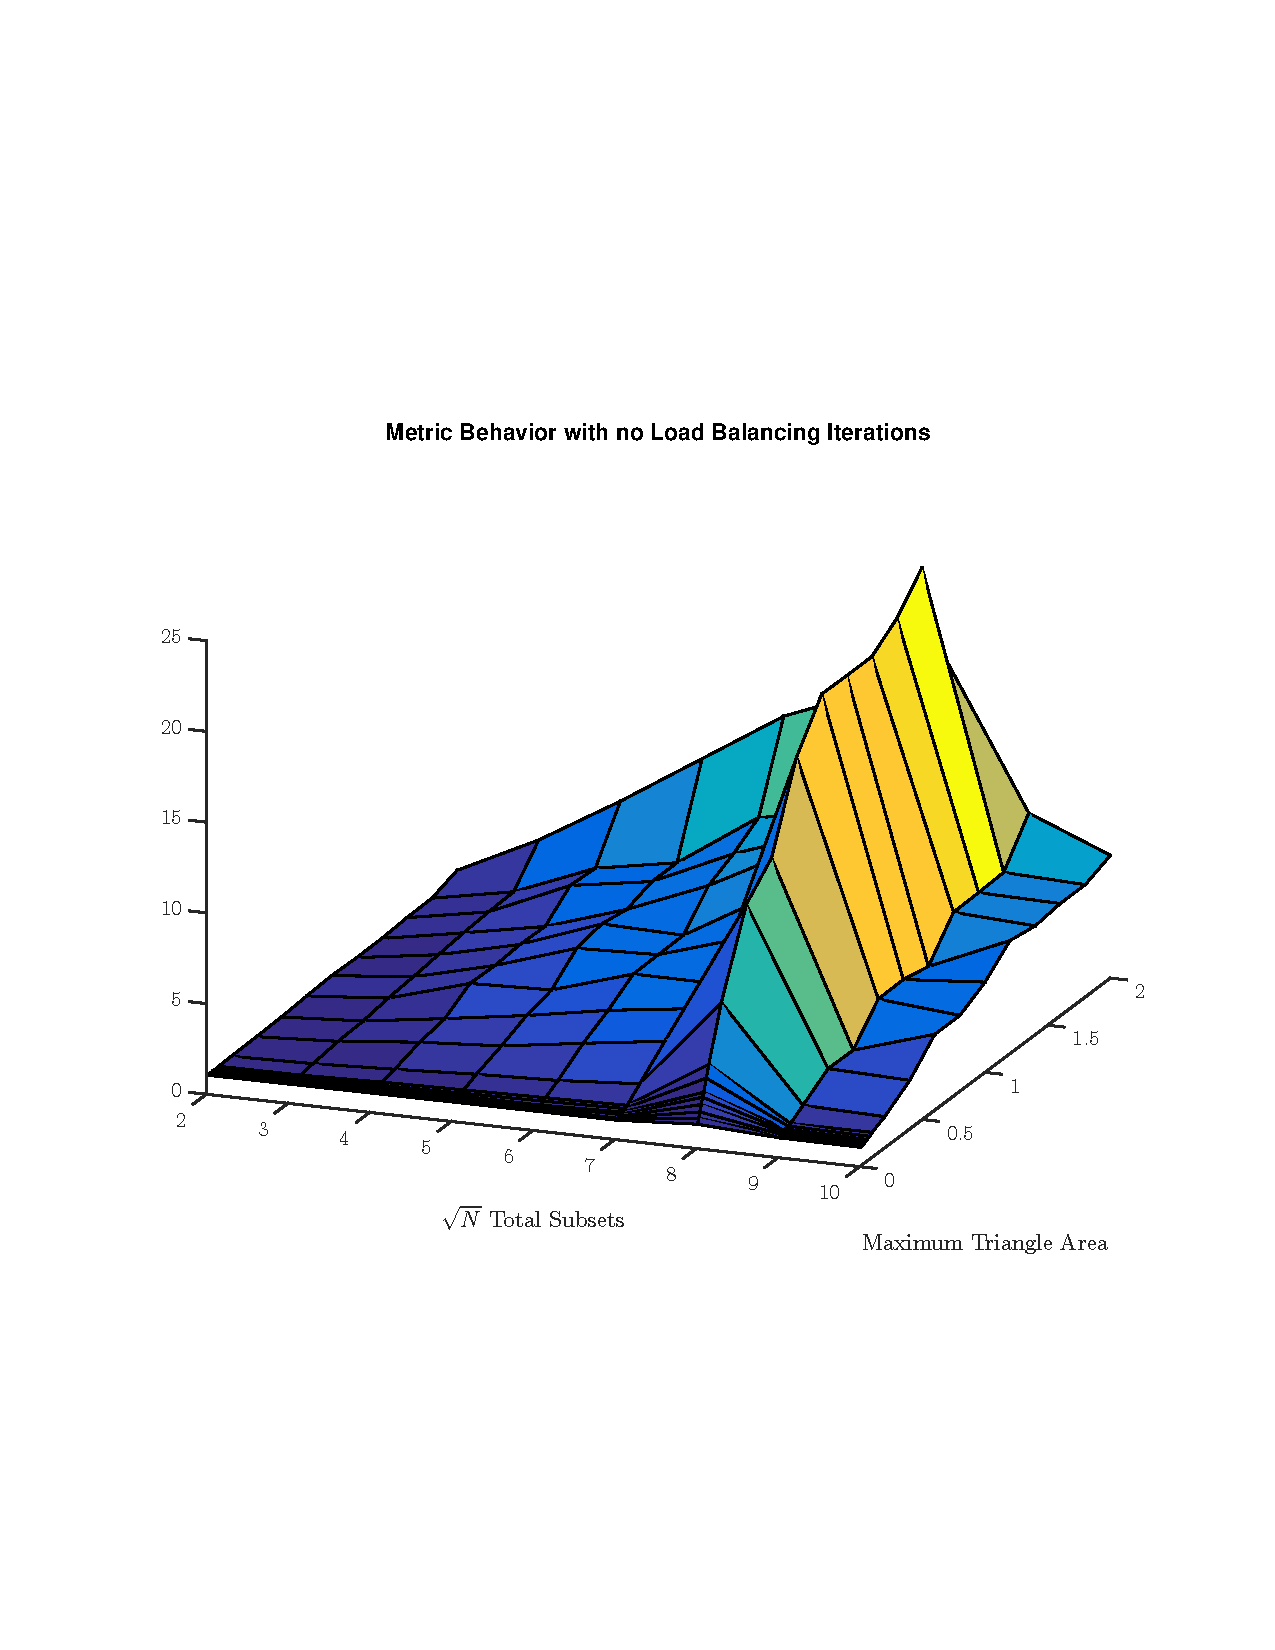
\includegraphics[scale=0.78, trim = 0cm 2cm 0cm 2cm,clip]{SameNoIter.pdf}
\captionof{figure}{The metric behavior of the second test case run with no load balancing iterations.}
\label{samenoiter}
\end{minipage}

Figure \ref{sameiter} shows the metric behavior for Fig. \ref{same}. The maximum metric is 3.9929 and occurs when Fig. \ref{same} is run with 10x10 subsets with a maximum triangle area of 1.8 cm\textsuperscript{2}. The minimum metric is 1.0024 and occurs when Fig. \ref{same} is run with 2x2 subsets with a maximum triangle are of 0.01 cm\textsuperscript{2}.

\noindent\begin{minipage}{\textwidth}
\centering
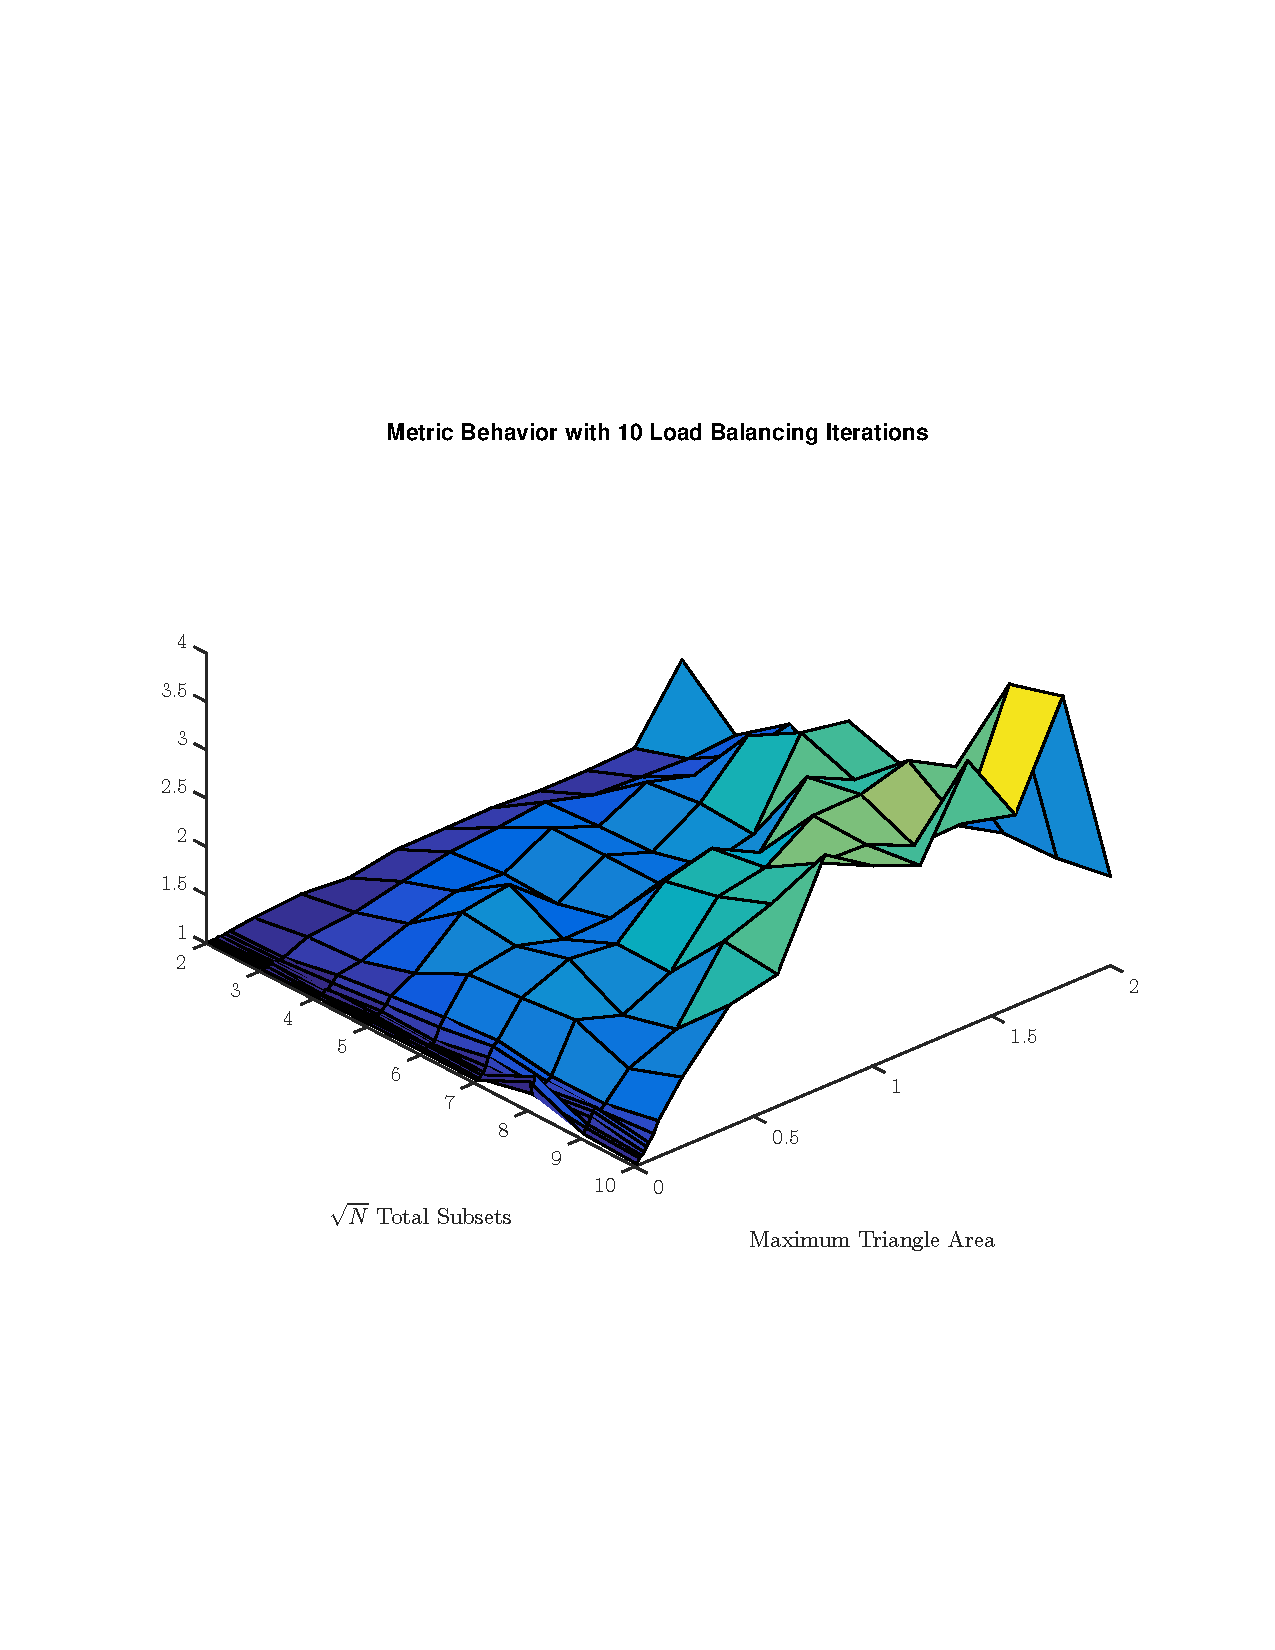
\includegraphics[scale=0.80, trim = 0cm 2cm 0cm 2cm,clip]{SameIter.pdf}
\captionof{figure}{The metric behavior of the second test case run with 10 load balancing iterations.}
\label{sameiter}
\end{minipage}

Figure \ref{samediff} shows the difference in metric behavior for Fig. \ref{same}. The maximum improvement has a value of 0.1090 and occurs for Fig. \ref{same} is run with 8x8 subsets with Triangle's coarsest possible mesh generation settings. The minimum improvement has a value of very close to 1.0 and occurs for many of the inputs. 

\noindent\begin{minipage}{\textwidth}
\centering
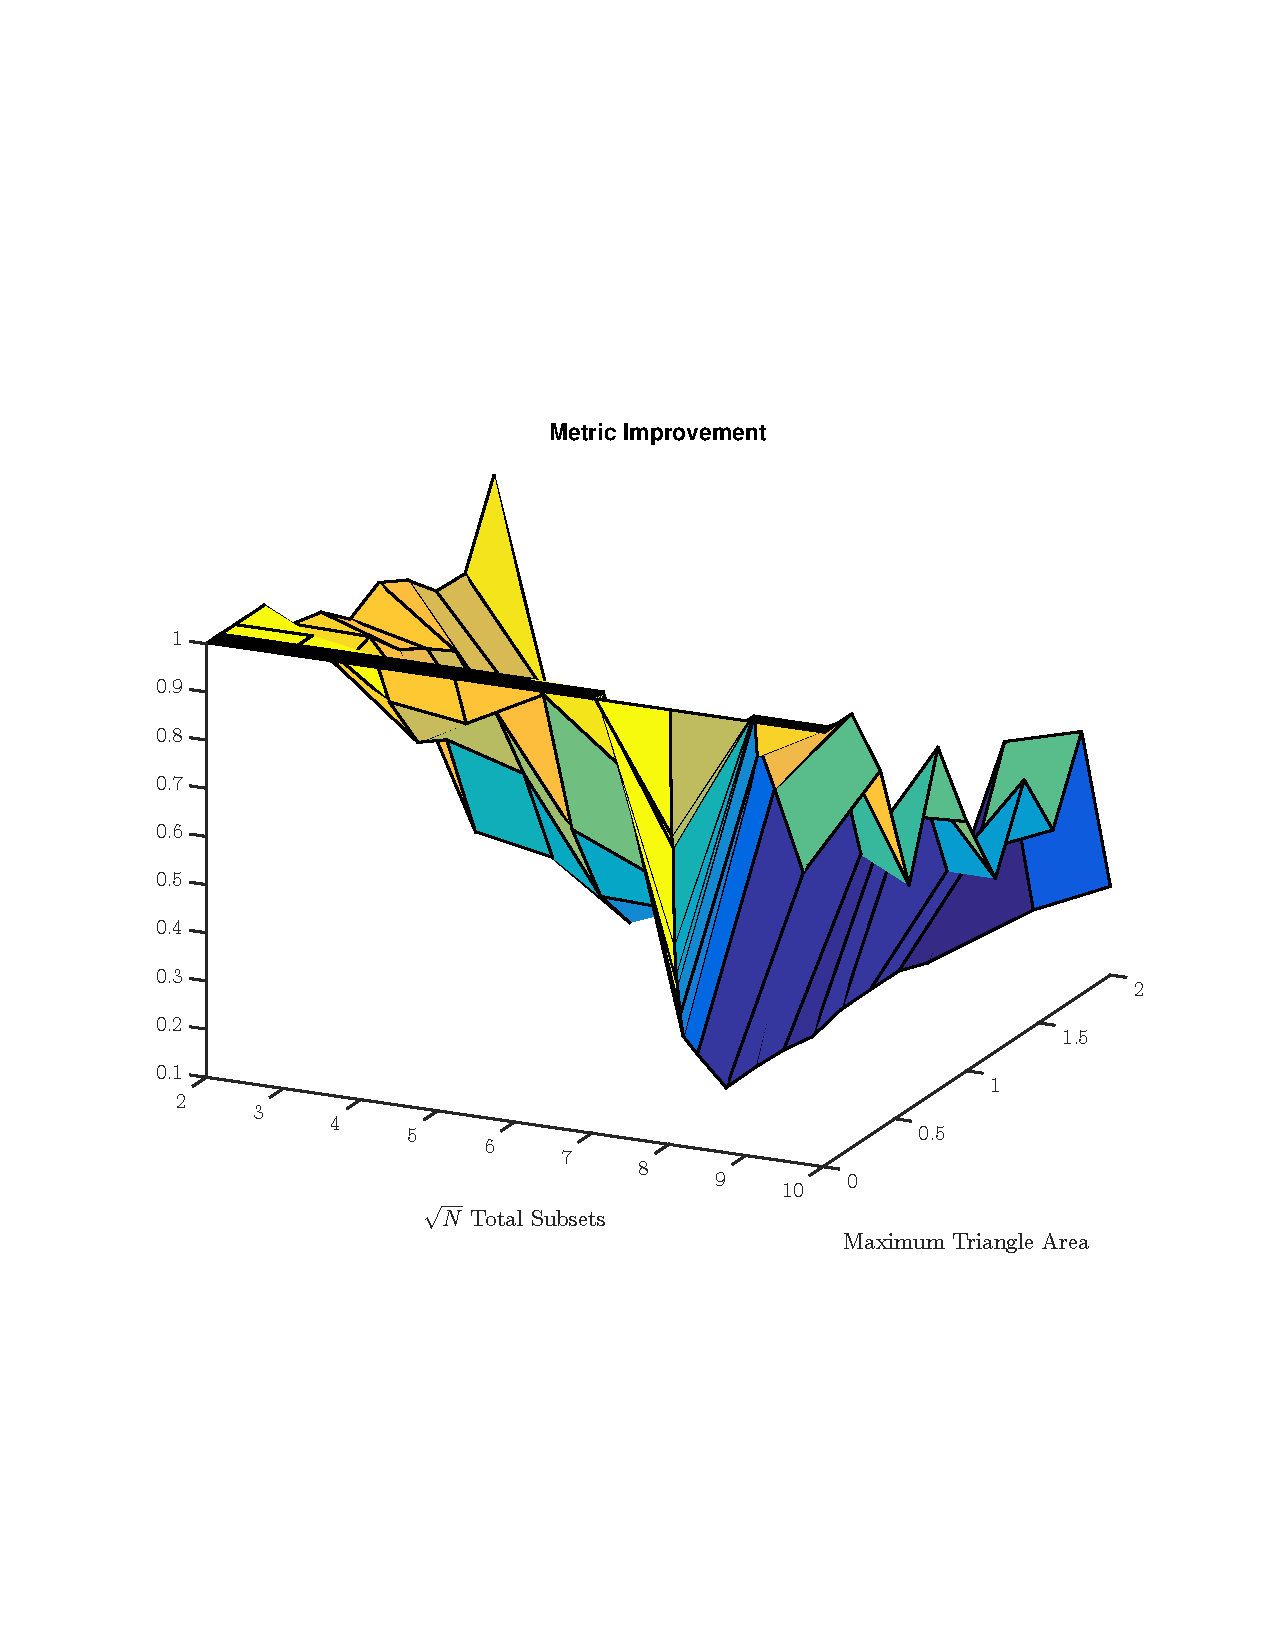
\includegraphics[scale=0.80, trim = 0cm 3cm 0cm 3cm,clip]{SameDiff.pdf}
\captionof{figure}{The difference in metric behavior of the second test case with no iteration and 10 iterations. The closer the z-value to zero, the better the improvement.}
\label{samediff}
\end{minipage}


\subsection{Solution Verification}

The test problem ran for solution verification is a pure absorbing slab with $\Sigma_a = 0.3 \text{cm}^{-1}$. It has reflecting boundary conditions on the top and the bottom, an incident isotropic flux on the left, and a vacuum boundary on the left. The reflecting boundaries are implemented to simulate an infinite slab in the y direction. The analytical solution to this problem is exponential \tcr{give the analytical expression and compare the ratio of analytical values (inlet/outlet)  with the numerical ones}, and with the flux placed on a logarithmic scale, we see the flux linearly decrease in the x direction. 

\noindent\begin{minipage}{\textwidth}
\centering
\hspace*{-3 cm}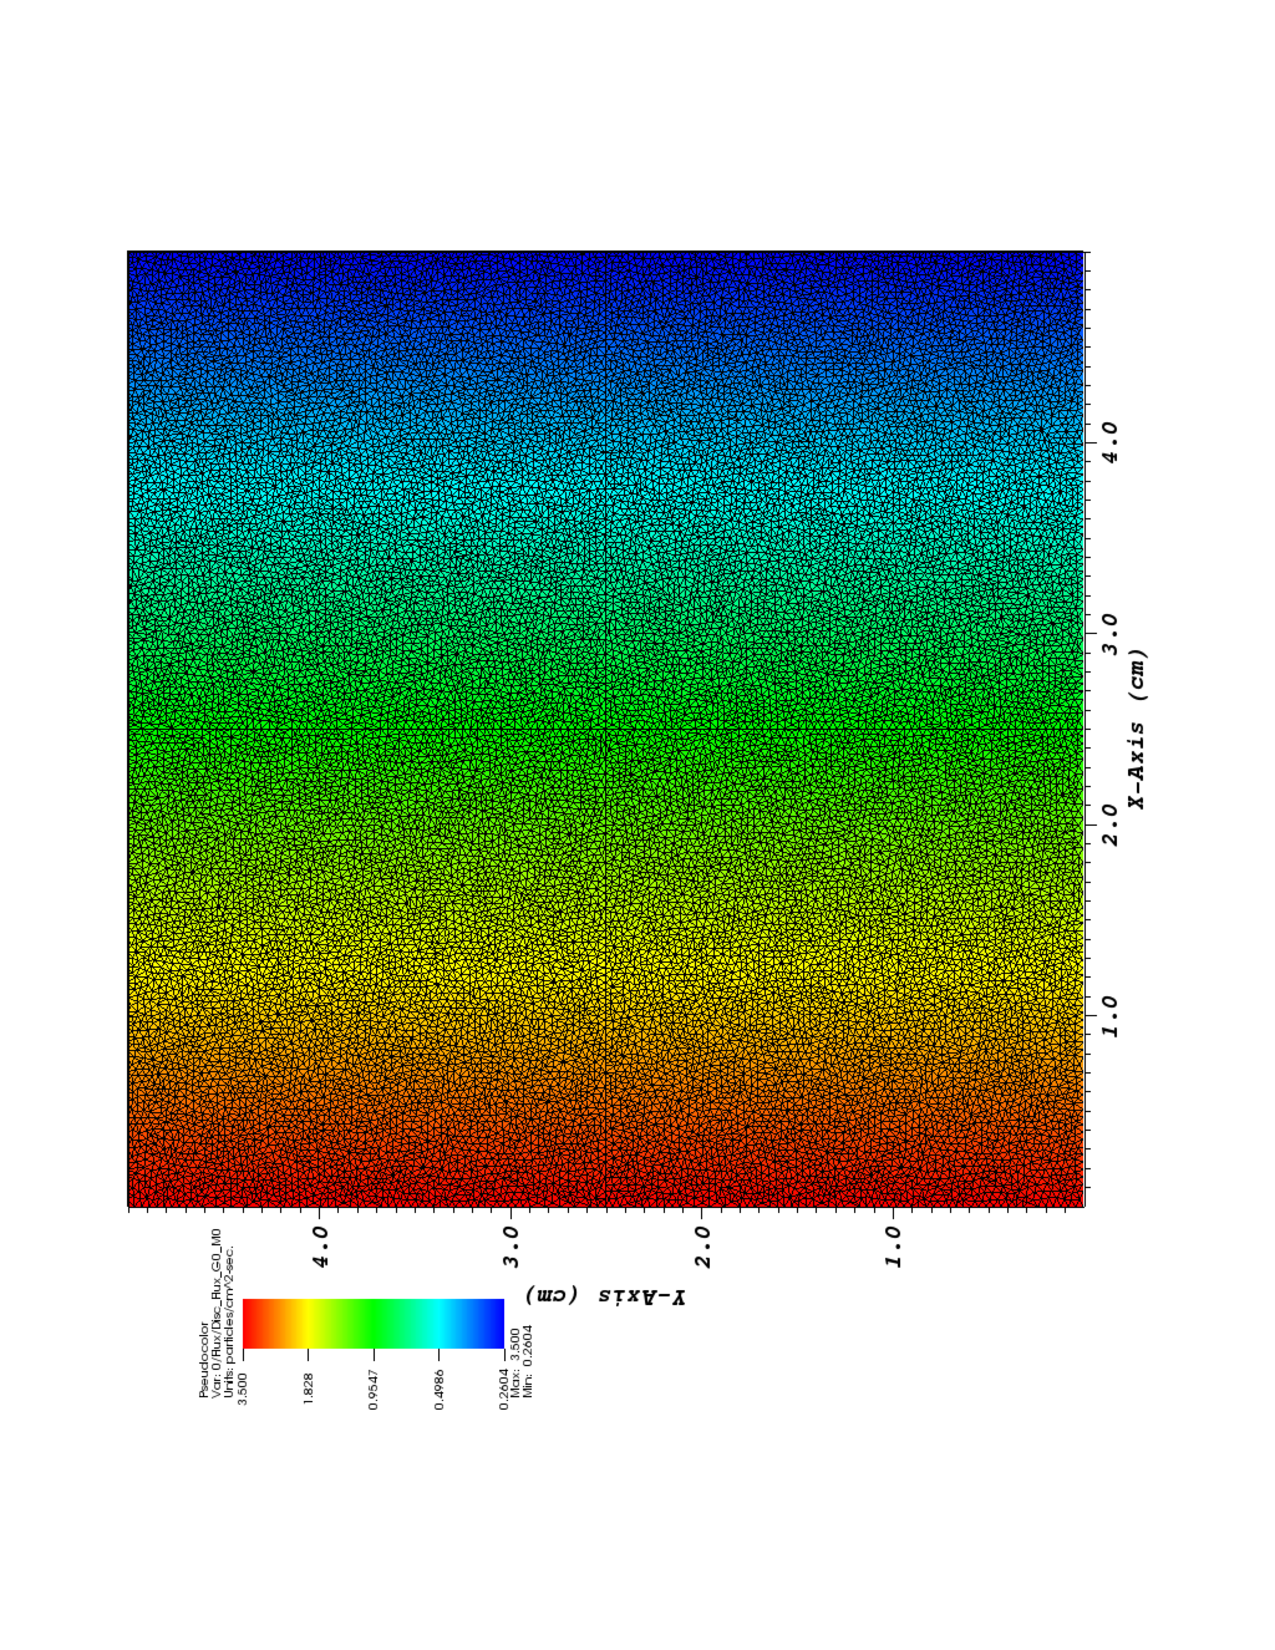
\includegraphics[scale=0.8,angle=-90]{PureAbsorberSolution.pdf}
\captionof{figure}{The solution of a pure absorbing slab.}
\label{pureabsorber}
\end{minipage}

\bibliographystyle{plain}
\bibliography{./Thesis}

\tcr{also use an optically thin domain with a pure scatterer, reflecting top/bottom, isotropic incident left, vacuum right, and verify that the solution is a straight line and compare left/right values with the known analytical solution}
\end{document}